\documentclass[letterpaper]{article} % DO NOT CHANGE THIS
% AAAI-27 Author Kit (official, https://aaai.org/authorkit27/, AuthorKit27.zip, aaai2027.sty dated 2026-10-21).
% AAAI anonymous workshop manuscript.
\usepackage[submission]{aaai2027}  % DO NOT CHANGE THIS
\usepackage[hyphens]{url}  % DO NOT CHANGE THIS
\usepackage{graphicx} % DO NOT CHANGE THIS
\urlstyle{rm} % DO NOT CHANGE THIS
\def\UrlFont{\rm}  % DO NOT CHANGE THIS
\usepackage{natbib}  % DO NOT CHANGE THIS AND DO NOT ADD ANY OPTIONS TO IT
\usepackage{caption} % DO NOT CHANGE THIS AND DO NOT ADD ANY OPTIONS TO IT
\frenchspacing  % DO NOT CHANGE THIS
\usepackage{algorithm}
\usepackage{algorithmic}
\usepackage{booktabs}
\usepackage{array}
\usepackage{amsmath}
\usepackage{placeins} % \FloatBarrier keeps appendix floats in their sections
\pdfinfo{
/TemplateVersion (2027.1)
}
\setcounter{secnumdepth}{2} % Section numbers enabled (permitted by the template: 0, 1 or 2).

\title{BrickForma: Crystallizing Large-Model Geometric Knowledge into a Small Language Model for Text-to-Brick Assembly}
\author{Anonymous submission}
\affiliations{}


\begin{document}
\maketitle
\begin{abstract}
Geometric spatial reasoning underlies applications from robotics to automated design, yet the ability of large language models (LLMs) to turn a verbal description into a physically connected three-dimensional assembly remains largely underexplored. Brick assembly is a demanding constructive probe of this ability: a short, underspecified prompt leaves dimensions, proportions, and part layout implicit, and a valid answer must match the semantic intent of the prompt while completing this geometry with discrete pieces that interlock through studs. We study this setting as the \textsc{Text-to-Brick} task and present BrickForma, a framework that crystallizes the geometric knowledge of large language models into a compact model for this task. Parametric programs written with large language model assistance generate 80,000 source voxel models across 21 categories on a $48^3$ grid, each described at five levels of detail, yielding approximately 400,000 caption records that tie varying amounts of language to shared geometry. A voxel-to-brick conversion pipeline with connection analysis and local retiling turns these shapes into geometrically checked brick targets, on which we fine-tune Qwen3-1.7B with low-rank adaptation to predict brick dimensions and positions from text. A mixed-integer linear programming stage then seeks an exact cover of the voxel target reconstructed from these predictions with a single stud-connected component. On 265 matched prompts spanning five description levels, the raw BrickForma outputs achieve the highest aggregate mean VQAScore (0.1079), PE (0.1572), and SigLIP2 (0.0565). Their mean invalid-placement ratio is 0.81\%, compared with 0.00\% for BrickGPT and 17.88\% for BrickNet. These results suggest that executable programs and checked geometric data are an effective route for carrying spatial knowledge from large models into a 1.7B-parameter one.
\end{abstract}


\begin{figure*}[t]
\centering
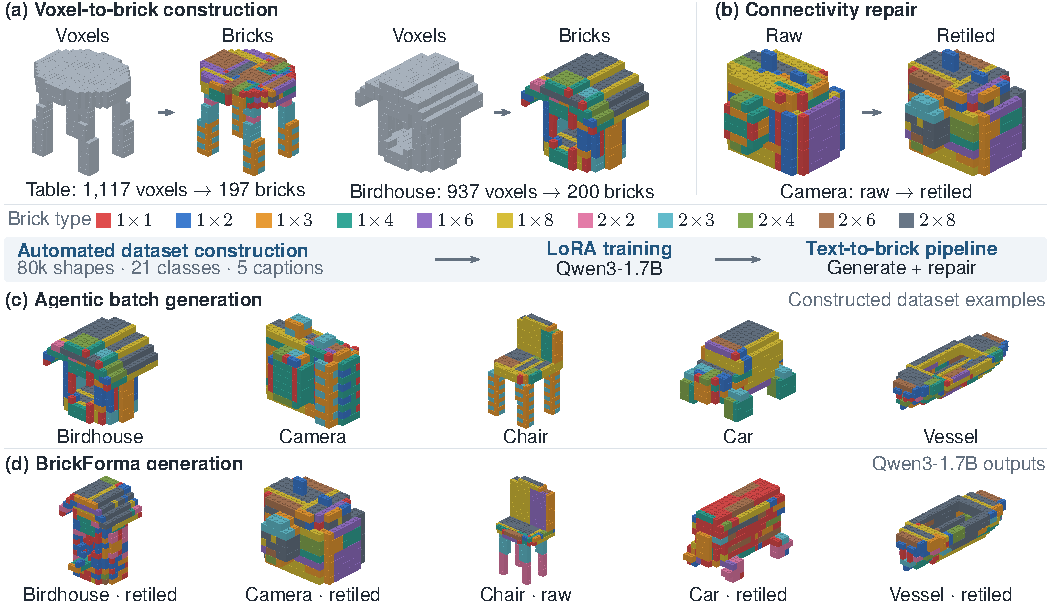
\includegraphics[width=\textwidth]{figure1.pdf}
\caption{BrickForma overview. (a) Source voxels are converted into rectangular bricks. (b) Raw predictions are retiled to repair connectivity. (c) Brick layouts constructed from programmatically generated voxels. (d) Outputs of the fine-tuned Qwen3-1.7B pipeline. Colors encode brick type independent of orientation; they are visualization labels, not predicted appearance. Voxels are shown in gray.}
\label{fig:teaser}
\end{figure*}

\section{Introduction}
Spatial reasoning and geometric understanding are fundamental to human cognition and to artificial intelligence, supporting applications from robotics and navigation to computer-aided design. As large language models (LLMs) have matured, a growing body of work asks whether they can reason about shape, position, and transformation. Recent benchmarks probe LLMs' ability through paper folding and unfolding~\cite{zhou2026paperfolding} and geometry expressed as procedural drawing code~\cite{luo2026geogrambench}, and each reports pronounced deficiencies in current models. These studies largely assess spatial reasoning by asking a model to select or compute an answer. A complementary and less examined question is whether a language model can \emph{construct}: given only words, can it produce a three-dimensional object whose parts are correctly sized, correctly placed, and physically joined?

Brick assembly makes this question concrete. A concise request such as \emph{a simple chair} identifies an object category while leaving its dimensions, proportions, and part layout largely unspecified. Answering it requires three coupled forms of geometric spatial reasoning. The model must complete the missing geometry from prior knowledge of what the object looks like. It must discretize that geometry into pieces of fixed dimensions at integer positions on a grid. And it must respect the difference between spatial adjacency and stud connectivity, since pieces that touch side by side do not hold together unless they interlock vertically through studs.

We refer to this setting as the \textsc{Text-to-Brick} task: the translation from a natural-language description, at any level of detail, to a set of brick placements that reproduces the described shape as a single connected assembly. Because every output can be checked for coverage, bounds, and connectivity, the task provides a verifiable test of whether linguistic knowledge has become spatial structure.

Prior work has established that language models can be trained for this task. BrickGPT~\cite{brickgpt} learns autoregressive brick-placement sequences and incorporates validity checks with physics-aware rollback during inference. BrickNet~\cite{bricknet} adopts a graph-based representation supporting a broader range of parts and connection types. Two questions remain open alongside these advances. \textbf{(Q1) How well do generators translate \emph{limited} linguistic information into object geometry?} In our five-level benchmark (Table~\ref{tab:levels}), BrickNet obtains lower mean VQAScore, PE, and SigLIP2 than BrickForma at the two shortest description levels, L1 and L2, a gap that only level-wise evaluation makes visible. \textbf{(Q2) Where should the geometric knowledge needed to answer concise requests come from?} Large models hold broad knowledge of object proportions and part structure, but that knowledge is implicit and their outputs carry no structural guarantee. Whether it can be transferred to a compact model in a form that can be inspected and checked has received limited attention.

We present BrickForma, which addresses both questions by \emph{crystallizing} large-model geometric knowledge into a small model through executable programs rather than through the large model's direct outputs. With GPT-6.1 Sol assistance, we develop parametric programs that vary object proportions, part dimensions, openings, and support arrangements to synthesize voxel shapes in batches. In this form, what a large model knows about a category becomes explicit and executable: each program fixes the structure of an object family and exposes its geometric degrees of freedom as parameters, so every generated shape is exact by construction. The source collection contains 80,000 models across 21 categories on a $48^3$ grid. Each model is paired with five levels of bilingual description that progressively introduce structural, geometric, proportional, and appearance information. The resulting approximately 400,000 caption records link concise requests and detailed specifications to shared geometry, so that a model trained on them learns to supply at the shortest level the geometric details that the longest level states outright.

Turning voxel shapes into brick targets is where spatial adjacency and stud connectivity must be separated. A connected voxel volume can be tiled by pieces that touch side by side without connecting through studs. Our conversion pipeline combines same-color tiling, connection analysis, and local bridging and retiling to construct geometrically checked target layouts, with changes to source voxels recorded in derived models. The integrated dataset release includes 79,301 models passing its dataset-level geometric checks. We fine-tune Qwen3-1.7B~\cite{qwen3} with low-rank adaptation~\cite{lora} on caption--placement pairs to predict brick dimensions and spatial positions. The knowledge transfer therefore passes through three inspectable stages, from programs to checked brick layouts to a 1.7B-parameter generator, and the small model never trains on an unverified large-model output.

Geometric reconstruction complements the small model's predictions with explicit structural enforcement. From the supported, in-bounds portions of predicted placements, the pipeline forms a voxel union and uses mixed-integer linear programming to seek an exact-cover layout forming a single stud-connected component. Independent coverage and connectivity checks verify the reconstructed result. This design assigns the two halves of the task to the components suited to them: the language model decides what shape a description denotes, and the solver decides how that shape holds together.

We evaluate BrickForma against BrickGPT and BrickNet on 265 shared Group B prompts spanning five description levels. The raw BrickForma outputs attain the highest aggregate mean VQAScore, PE, and SigLIP2, with a mean invalid-placement ratio of 0.81\%. Reporting all five levels reveals that BrickForma leads PE and SigLIP2 even at L1, where BrickGPT has the highest mean VQAScore.

In summary, the main contributions of this work are as follows:

\noindent\textbf{Crystallizing large-model geometric knowledge into a small model without human-verified data.}
We propose a data generation pipeline for transferring geometric and spatial knowledge from large language models to a compact model: the large model's knowledge is externalized as executable parametric programs, converted into geometrically validated training data, and distilled into a 1.7B-parameter model without relying on human verification. On Group B, the raw model's mean VQAScore is 16.5\% higher than that of BrickGPT, the stronger baseline on this metric (0.1079 versus 0.0926).

\noindent\textbf{A multi-level dataset that enables experimental validation of small language model alignment across various levels of descriptive detail.}
With our LLM-assisted parametric data construction pipeline, we generated 80,000 source voxel models. Each voxel model is paired with five levels of textual description and geometrically validated brick targets. We fine-tuned Qwen3-1.7B on this dataset and carried out level-wise evaluation against BrickGPT and BrickNet to assess text--image alignment and invalid placements across descriptions ranging from concise prompts to detailed specifications. BrickForma leads all three alignment metrics at L2--L5.


\begin{figure*}[t]
\centering
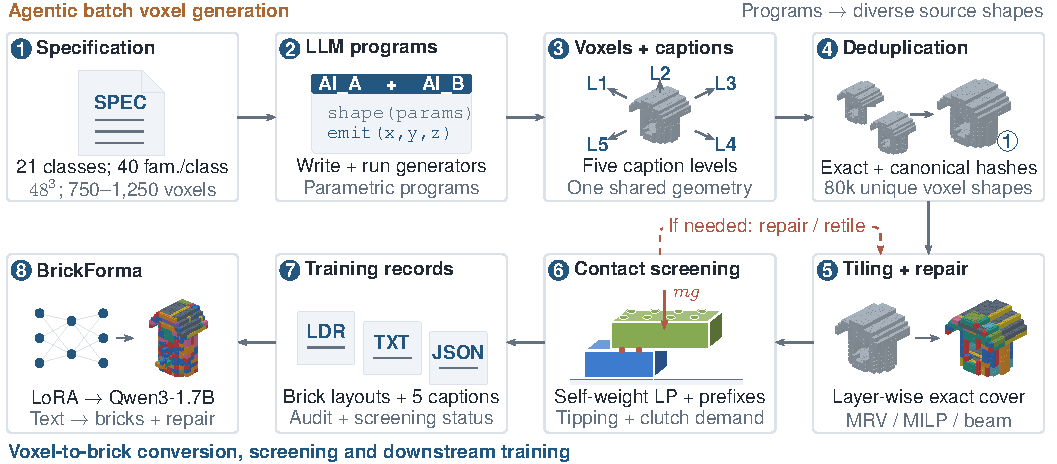
\includegraphics[width=\textwidth]{figure2.pdf}
\caption{Data-construction workflow. Parametric programs written by GPT-6.1 Sol through agentic batch generation produce voxel shapes and captions, followed by deduplication, same-color tiling, local repair, and audited export for fine-tuning. Contact screening is recorded separately. The dashed arrow denotes repair or retiling when needed. Screening is distinct from a guarantee of physical stability. Brick colors follow the legend in Figure~\ref{fig:teaser}.}
\label{fig:data-workflow}
\end{figure*}

\section{Related Work}
\paragraph{Spatial reasoning and constructive generation.}
Paper-folding and program-to-geometry benchmarks test how models derive geometric answers from visual or symbolic information~\cite{zhou2026paperfolding,luo2026geogrambench}. Brick assembly asks for an executable spatial output: a collection of discrete placements that can be checked for coverage, overlap, and connection. MeshGPT and LLaMA-Mesh represent 3D geometry as token sequences~\cite{meshgpt,llamamesh}. Our sequence encodes rectangular footprints and absolute grid positions.

\paragraph{Brick assembly and stability.}
Prior work treats brick assembly as graph generation, sequential construction, or structure understanding~\cite{thompson2020lego,brickbybrick,breakandmake}. BrickGPT uses autoregressive placement sequences and physics-aware rollback~\cite{brickgpt}. BrickNet represents a wider range of parts and connectors with an assembly graph~\cite{bricknet}. BrickForma imposes a single stud-connected component by reconstructing the predicted volume. Force-balance screening, as studied by StableLego~\cite{stablelego}, requires a separate mechanical model.

\paragraph{Procedural supervision.}
Procedural generation offers control over shape variation and scale~\cite{infinigen}. SpatialVLM uses synthetic supervision to teach spatial relations to a vision--language model~\cite{spatialvlm}. BrickForma uses a language model to author executable generators, checks their geometric outputs algorithmically, and trains a text-only model on the resulting text--placement pairs using LoRA~\cite{lora}.

\section{From Programs to Checked Training Data}
\label{sec:dataset}
\subsection{Parametric Programs and Shared Geometry}
GPT-6.1 Sol assists in writing parameterized programs for 21 object categories. Each program defines an object family through part dimensions, proportions, openings, and support arrangements. Executing the programs gives 80,000 source voxel models in two 40,000-model shards on a $48^3$ grid, with 750--1,250 occupied cells per object. Exact and canonical occupancy hashes over 48 axis/sign transforms found no cross-shard duplicates. Geometry plans and version identifiers accompany the records (Figure~\ref{fig:data-workflow}).

BrickMore-48 pairs each shape with five bilingual descriptions. L1 expresses the object and its main parts, while progressively richer descriptions add structure, proportions, appearance, and views. The geometry is shared by all five levels, so the same target provides supervision for both concise and detailed requests. Appendix~\ref{app:dataset} gives a birdhouse example.

\subsection{Voxel-to-Brick Conversion}
The conversion tiles each layer with same-color rectangular footprints and inspects the resulting stud components. Local bridging and retiling address ungrounded components, with edits recorded against the source voxels. The retile release raises the geometry-pass count from 65,503 to 79,298, recovering 13,795 failures. Across the corpus it adds 228,582 and removes 125 voxels, and 31,532 passing models require no edits.

The release checks that the target voxels are six-neighbor connected, every brick component is grounded, and brick placement exactly covers the derived target. Several individually grounded brick components may pass these release checks. Inference uses a stricter single-component constraint. Contact-based gravity screening records a separate outcome (Appendix~\ref{app:dataset}).

\subsection{Integrated Release and Training Corpus}
The full retile release contains 702 geometry failures. A revised batch-B piano release passes all 1,905 slots where the full retile release passed 1,902, giving a report-derived integrated count of $79{,}298-1{,}902+1{,}905=79{,}301$. Table~\ref{tab:training-data} reports the release and recorded fine-tuning counts.
\begin{table}[t]
\centering
\small
\setlength{\tabcolsep}{4pt}
\begin{tabular}{lr}
\toprule
\multicolumn{2}{l}{\emph{Dataset (release reports)}} \\
\midrule
Source models / categories / grid & 80,000 / 21 / $48^3$ \\
Bilingual caption records & 400,000 \\
Failing in full retile release & 702 (0.88\%) \\
Passing in full retile release & 79,298 \\
Piano models restored by revised release & 3 \\
Integrated passing models & 79,301 \\
\midrule
\multicolumn{2}{l}{\emph{Fine-tuning corpus}} \\
\midrule
(model, English caption) samples & 396,610 \\ % Training manifest confirmation pending
Training / validation samples & 356,955 / 39,655 \\
Tokens over 3 epochs & 2,228,044,818 \\ % Training manifest confirmation pending
\bottomrule
\end{tabular}
\caption{Dataset and fine-tuning corpus. The two blocks are counted separately: the upper block from the dataset release reports, the lower block as recorded for the fine-tuning run.}
\label{tab:training-data}
\end{table}

\begin{algorithm}[tb]
\caption{BrickForma inference and retiling}
\label{alg:inference-retiling}
\small
\begin{algorithmic}[1]
\REQUIRE prompt $c$; fine-tuned model $\theta$; library $\mathcal{L}$ (20 footprints); seeds $S=(42,104,2026)$; MILP tiers $T=(12,60,180)$\,s
\ENSURE $(B_{\mathrm{out}}, \textit{status})$, $\textit{status}\in\{\textsc{Success},\textsc{Draft},\textsc{Failed}\}$
\STATE $B \gets \emptyset$; $A \gets \emptyset$
\FOR{$s \in S$}
  \STATE $(B_s,\textit{rep}) \gets \mathrm{Parse}(\theta.\mathrm{Generate}(c,\ \mathrm{seed}{=}s))$
  \STATE $A \gets A \cup \{(B_s,\textit{rep})\}$
  \IF{$\textit{rep}.\mathrm{complete} \land \textit{rep}.\mathrm{valid}$}
    \STATE $B \gets B_s$; \textbf{break}
  \ENDIF
\ENDFOR
\IF{$B=\emptyset$}
  \IF{no completed draft in $A$}
    \RETURN $(\emptyset,\ \textsc{Failed})$
  \ENDIF
  \STATE $B \gets \arg\min_{\text{completed } a\in A} \mathrm{Err}(a)$
\ENDIF
\IF{$\mathrm{Err}(B)=0 \land \mathrm{StudComponents}(B)=1$}
  \RETURN $(B,\ \textsc{Success})$ \COMMENT{keep a valid connected raw layout}
\ENDIF
\STATE $C \gets \mathrm{UnionVoxels}(B;\ \mathcal{L},\ 48^3)$ \COMMENT{clip; overlaps count once}
\FOR{$\tau \in T$}
  \STATE $B^{*} \gets \mathrm{MILP\text{-}SingleStudCover}(C,\ \tau)$
  \IF{$B^{*}\neq\emptyset \land \mathrm{Audit}(B^{*},C)$}
    \RETURN $(B^{*},\ \textsc{Success})$
  \ENDIF
\ENDFOR
\STATE $\mathrm{QueueReseed}(c)$
\RETURN $(B,\ \textsc{Draft})$ \COMMENT{unsolved: keep raw draft}
\end{algorithmic}
\end{algorithm}

\begin{figure*}[t]
\centering
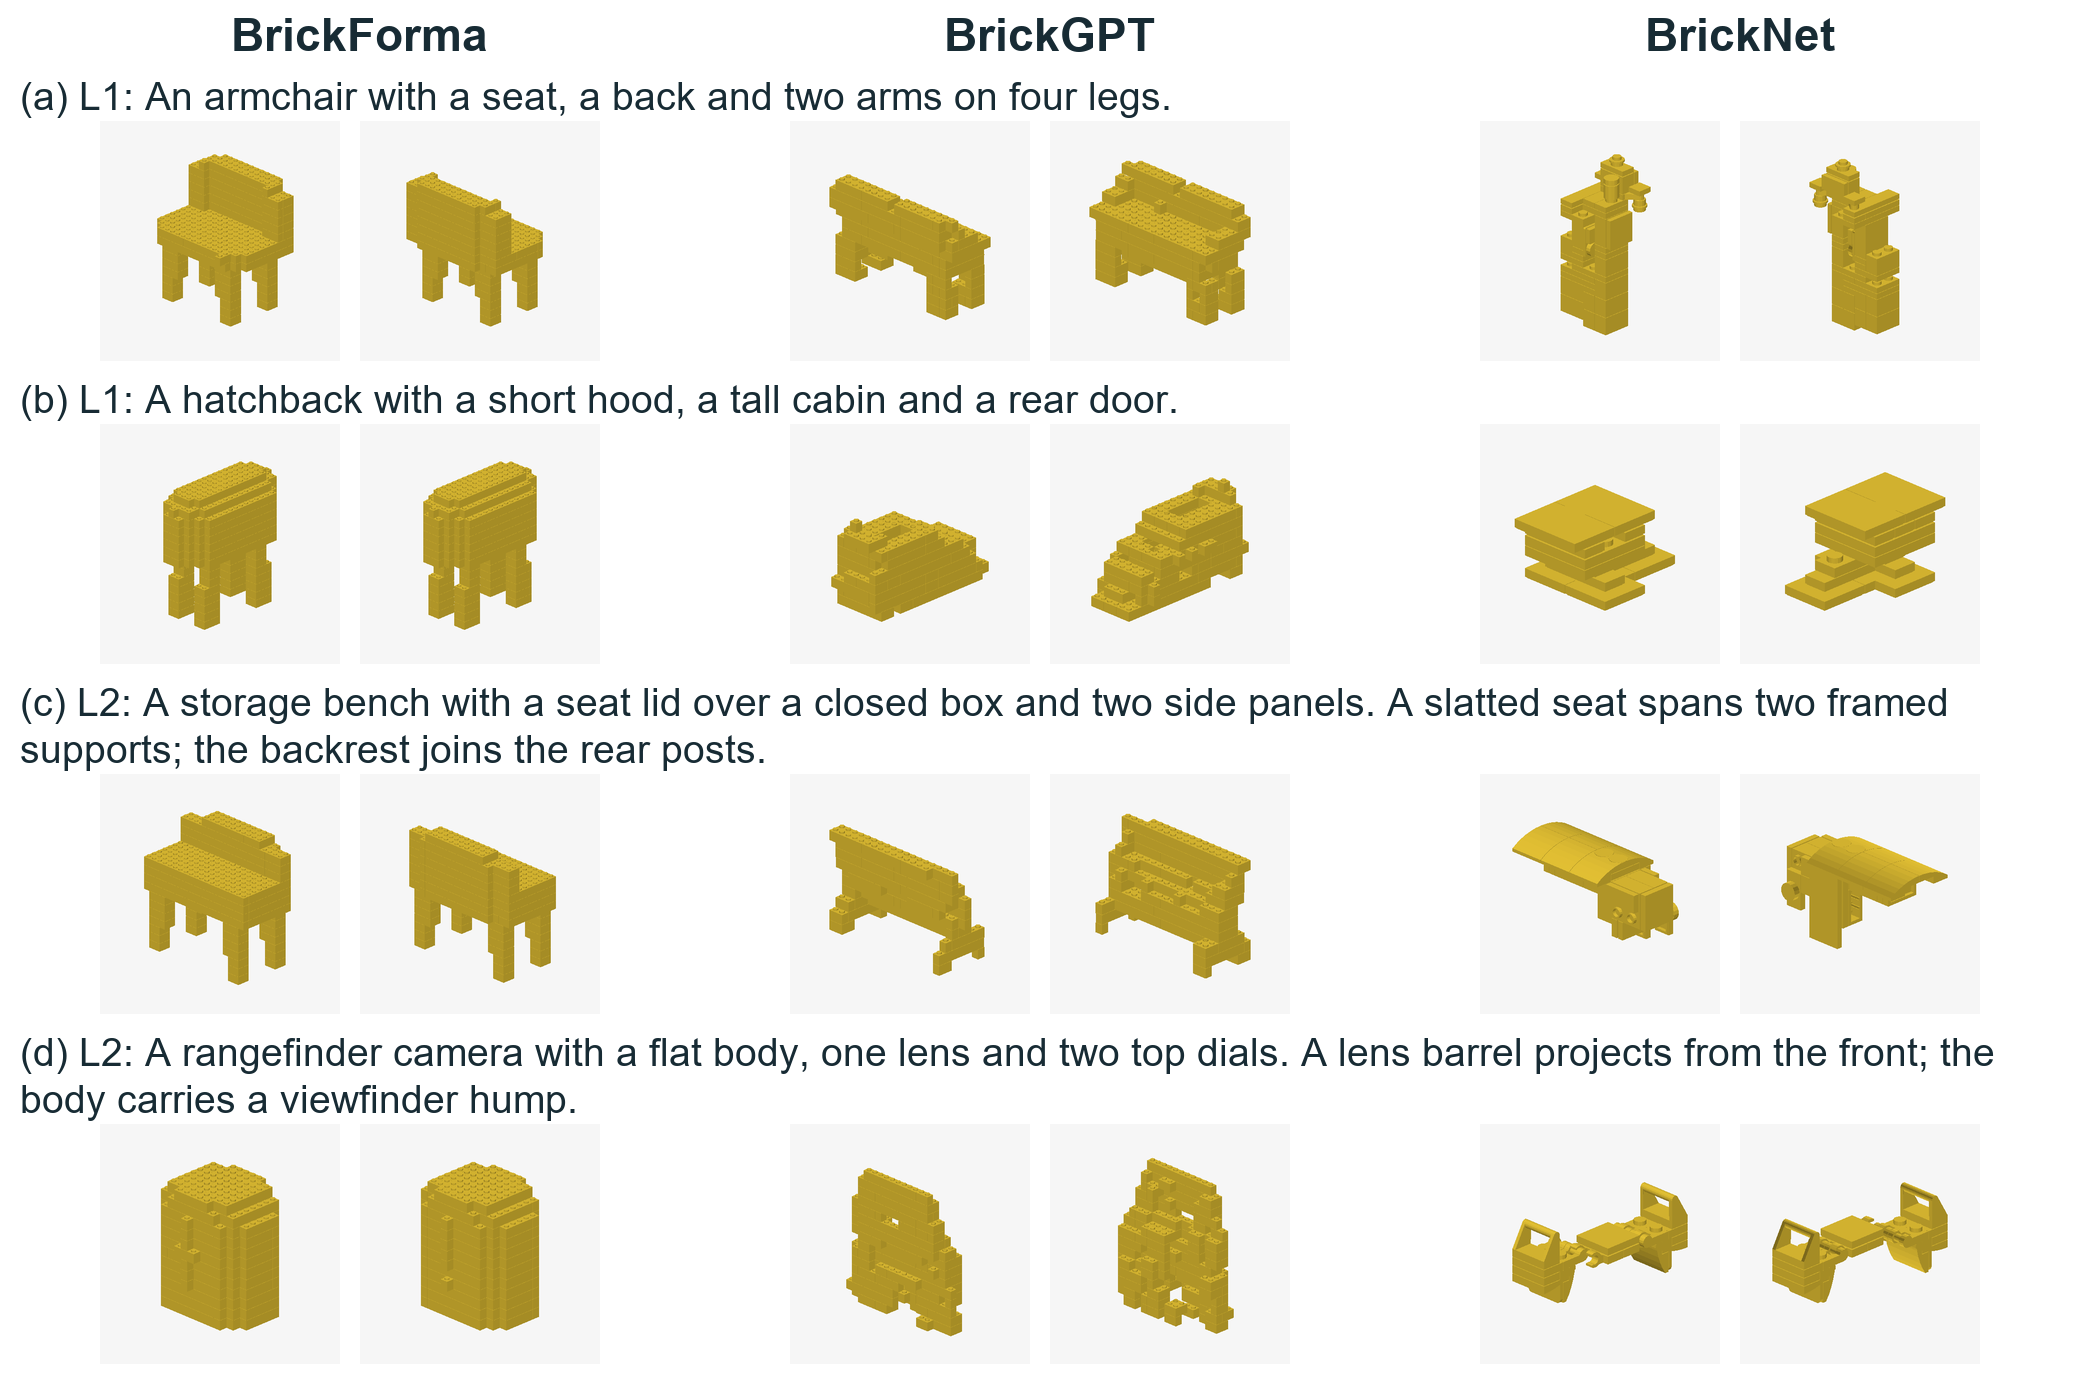
\includegraphics[width=\textwidth]{figures/matched_short_prompts_20261116.png}
\caption{Four matched Group B examples with the same prompts, render settings, and azimuths ($45^\circ$ and $225^\circ$) across systems. The highest VQAScore belongs to BrickForma for the chair and bench, BrickGPT for the hatchback, and BrickNet for the camera.}
\label{fig:gallery}
\end{figure*}


\section{From Text to a Connected Assembly}
\label{sec:model}
\subsection{Learning a Placement Sequence}
\label{sec:training}
We fine-tune Qwen3-1.7B with LoRA on English L1--L5 captions and their checked brick layouts. A model-level 9:1 split keeps descriptions of the same shape together. The $48^3$ grid uses 20 oriented footprints (11 brick sizes up to planar rotation). The instruction lists the allowed dimensions, and the target gives one placement per line, such as $2{\times}4\ (x,y,z)$. Dimensions are serialized Y-first, then X. The sequence describes geometry and omits color.

Fine-tuning follows the BrickGPT Qwen3 script~\cite{brickgpt} (Table~\ref{tab:finetune-config}). Unpacked sequences preserve caption boundaries. The run reached 133,860 steps in 25.3 hours on eight GPUs. Validation loss reached 0.0308 at step 79,000, the released checkpoint, and 0.0339 at the end of epoch 3. Appendix~\ref{app:training} records the validation checkpoints.
\begin{table}[t]
\centering
\small
\setlength{\tabcolsep}{3pt}
\begin{tabular}{@{}l>{\raggedright\arraybackslash}p{0.58\linewidth}@{}}
\toprule
Item & Value \\
\midrule
Base model & Qwen3-1.7B (bf16) \\
Adaptation & LoRA, $r=16$, $\alpha=32$, dropout $0.05$, all linear layers \\
Optimization & LR $10^{-4}$, cosine, 100 warm-up steps, 3 epochs \\
Batch / max length & effective 8 (8 GPUs $\times$ 1) / 8,192 \\
Hardware & DDP, 8$\times$RTX 4090D (24\,GB) \\
Released checkpoint & step 79,000 (best validation loss) \\
Software & transformers 4.51.3, trl 0.17.0, peft 0.15.2 \\
\bottomrule
\end{tabular}
\caption{Fine-tuning configuration (details in Appendix~\ref{app:training}).}
\label{tab:finetune-config}
\end{table}


\subsection{Reconstructing a Single Stud Component}
Algorithm~\ref{alg:inference-retiling} samples with thinking disabled, temperature $0.7$, top-$p$ $0.9$, and at most 8,192 new tokens. It tries seeds 42, 104, and 2026, keeping the first completed draft that passes the geometry validator or the completed draft with the fewest format, library, bounds, and overlap errors. A valid draft with a single stud component is returned as is.

For other drafts, the pipeline forms the in-bounds voxel union $C$ of supported placements, counting overlaps once. Mixed-integer linear programming (MILP) seeks an exact cover of $C$ with one stud-connected component at 12, 60, and 180 seconds. An accepted solution passes an independent audit of placement validity, coverage, and connectivity. If the budget is exhausted, the pipeline can retain the draft and queue a new seed. Recovery runs can sample additional seeds or extend the budget to 600 seconds. We call the drafts \emph{raw} and the accepted reconstructions \emph{retiled}.

\section{Comparative Evaluation}
\label{sec:eval}
\subsection{Setup and Metrics}
\label{sec:setup}
The November 16 evaluation contains 1,315 LDraw exports across two cohorts spanning 21 categories and five description levels. Group B is the main comparison: 265 shared prompts, 53 per level, with one delivered output per system per prompt. The BrickForma inputs are raw outputs generated with its Q8\_0 weights. Group A contains 260 matched prompts for BrickGPT and BrickNet (Appendix~\ref{app:eval}). We score all supplied exports in both cohorts.

We use uniform yellow material and render each export at $512{\times}512$ from eight orthographic azimuths at $45^\circ$ intervals and $25^\circ$ elevation. For each text--image metric we take the maximum over views, then average over prompts. VQAScore~\cite{vqascore} uses the first-token probability of \textquotedblleft Yes\textquotedblright\ from Qwen2.5-VL-7B-Instruct~\cite{qwen25vl}. PE~\cite{pe} uses cosine similarity of normalized embeddings, and SigLIP2~\cite{siglip2} uses the sigmoid of the image--text logit. We compute $P_{\mathrm{inv}}$ as the mean fraction of invalid placements per model in export order, using BrickNet's inset collision kernel~\cite{bricknet}.

\subsection{Performance across Description Levels}
Table~\ref{tab:levels} addresses Q1 by separating Group B into L1--L5. BrickForma leads PE and SigLIP2 at all five levels and VQAScore at L2--L5. At L1 (13.4 words on average), BrickGPT has a slightly higher VQAScore (0.1911 versus 0.1841). BrickGPT has the lowest mean $P_{\mathrm{inv}}$ at each level. Figure~\ref{fig:gallery} illustrates individual outcomes from the same comparison.
\begin{table*}[t]
\centering\small
\setlength{\tabcolsep}{3pt}
\begin{tabular}{lrrlrrrr}
\toprule
Level & $n$ & Words & System & $P_{\mathrm{inv}}\downarrow$ & VQAScore $\uparrow$ & PE $\uparrow$ & SigLIP2 $\uparrow$ \\
\midrule
L1 & 53 & 13.4 & BrickForma & 0.41\% & 0.1841 & \textbf{0.1409} & \textbf{0.0254} \\
 &  &  & BrickGPT & \textbf{0.00\%} & \textbf{0.1911} & 0.1323 & 0.0132 \\
 &  &  & BrickNet & 15.14\% & 0.0445 & 0.1032 & 0.0002 \\
\midrule
L2 & 53 & 26.4 & BrickForma & 0.78\% & \textbf{0.1651} & \textbf{0.1453} & \textbf{0.0241} \\
 &  &  & BrickGPT & \textbf{0.00\%} & 0.1354 & 0.1391 & 0.0206 \\
 &  &  & BrickNet & 17.74\% & 0.0579 & 0.1037 & 0.0013 \\
\midrule
L3 & 53 & 37.3 & BrickForma & 0.73\% & \textbf{0.1467} & \textbf{0.1479} & \textbf{0.0717} \\
 &  &  & BrickGPT & \textbf{0.00\%} & 0.1061 & 0.1396 & 0.0199 \\
 &  &  & BrickNet & 23.30\% & 0.0211 & 0.1075 & 0.0012 \\
\midrule
L4 & 53 & 52.3 & BrickForma & 1.38\% & \textbf{0.0239} & \textbf{0.1792} & \textbf{0.0914} \\
 &  &  & BrickGPT & \textbf{0.00\%} & 0.0198 & 0.1609 & 0.0487 \\
 &  &  & BrickNet & 18.68\% & 0.0023 & 0.1344 & 0.0016 \\
\midrule
L5 & 53 & 78.6 & BrickForma & 0.75\% & \textbf{0.0198} & \textbf{0.1727} & \textbf{0.0698} \\
 &  &  & BrickGPT & \textbf{0.00\%} & 0.0107 & 0.1575 & 0.0286 \\
 &  &  & BrickNet & 14.56\% & 0.0035 & 0.1379 & 0.0035 \\
\bottomrule
\end{tabular}
\caption{Group B means by description level. Each level contains 53 prompts per system. Words is the mean English word count. Bold marks the best mean.}
\label{tab:levels}
\end{table*}


\subsection{Aggregate Results}
\begin{table}[t]
\centering\small
\setlength{\tabcolsep}{3pt}
\begin{tabular}{lrrrr}
\toprule
System & $P_{\mathrm{inv}}\downarrow$ & VQAScore $\uparrow$ & PE $\uparrow$ & SigLIP2 $\uparrow$ \\
\midrule
BrickForma & 0.81\% & \textbf{0.1079} & \textbf{0.1572} & \textbf{0.0565} \\
BrickGPT & \textbf{0.00\%} & 0.0926 & 0.1459 & 0.0262 \\
BrickNet & 17.88\% & 0.0259 & 0.1173 & 0.0016 \\
\bottomrule
\end{tabular}
\caption{Group B means on 265 matched prompts. BrickForma uses delivered raw outputs. Bold marks the best mean.}
\label{tab:main}
\end{table}

BrickForma attains the highest mean VQAScore (0.1079), PE (0.1572), and SigLIP2 (0.0565) on Group B (Table~\ref{tab:main}). It exceeds BrickGPT on 188, 166, and 168 of 265 prompts for the three metrics, respectively. All six pairwise comparisons pass Holm correction under both paired tests (Appendix~\ref{app:eval}). The raw BrickForma exports have mean $P_{\mathrm{inv}}$ of 0.81\%, compared with 0.00\% for BrickGPT and 17.88\% for BrickNet.

\subsection{Geometry Before and After Reconstruction}
\label{sec:diagnostics}
We assess reconstruction on 110 raw/retiled pairs from the earlier 114-prompt comparison. Adjacent-layer footprint overlap defines stud contacts. After mapping exports to a grid with 20 LDU horizontal pitch and 24 LDU layer height and translating occupied cells to a common origin, all 110 pairs have equal voxel unions. The number with a single stud component rises from 18 to 110 (Table~\ref{tab:export-audit}).
\begin{table}[t]
\centering\small
\begin{tabular}{@{}lrr@{}}
\toprule
Export measure & Raw & Retiled \\
\midrule
Single stud component & 18/110 & 110/110 \\
Mean stud components & 4.29 & 1.00 \\
No body-cell overlap & 100/110 & 110/110 \\
\midrule
\multicolumn{3}{@{}l@{}}{Equal voxel unions after translation: 110/110} \\
\bottomrule
\end{tabular}
\caption{Earlier export audit of 110 matched raw/retiled pairs. Union equality uses translation normalization.}
\label{tab:export-audit}
\end{table}

Across these pairs $P_{\mathrm{inv}}$ falls from 0.1897\% to 0.0000\%, while mean part count rises from 178.7 to 421.2. In the separate 525-prompt diagnostic cohort, 46 raw layouts (8.8\%) have a single stud component, and all 525 final layouts pass both geometry checks after the reported recovery procedure (Appendix~\ref{app:eval}).

\section{Limitations and Discussion}
The transfer described in Q2 combines program design, geometric checks, and supervised fine-tuning. Isolating the contribution of large-model program authoring would require controls with alternative generators and matched training budgets.

The delivered systems use different inference settings and part libraries. Description levels vary in both content and length, and long descriptions may be truncated (Appendix~\ref{app:eval}). Alignment scores describe rendered appearance, while $P_{\mathrm{inv}}$ measures collisions under the stated file order. Physical stability and assembly-order feasibility require separate validation.

\section{Conclusion}
BrickForma uses executable programs to synthesize voxel shapes and converts them into checked training layouts for Qwen3-1.7B. On the 265 matched prompts, its raw exports lead all three alignment metrics in aggregate. Earlier reconstruction audits show that exact-cover repair can preserve the predicted volume while supplying connections that the model frequently misses.

\bibliography{references}
\FloatBarrier
\appendix
\section{Technical Appendix: Dataset Details}
\label{app:dataset}
The historical figures and tables in this appendix retain the supplied measurements and model renders, with labels translated into English. They use release-specific versions and criteria and are not substitutes for the integrated statistics or the current main comparison.

\emph{Caption example.} The five captions of one model share a prefix and add detail level by level. The L1 prompt is \textquotedblleft An oval birdhouse with curved roof, enclosed room and front entrance.\textquotedblright\ Its L5 description is: ``An oval birdhouse with curved roof, enclosed room and front entrance. The protective roof joins the walls; the circular front entrance reaches a real interior cavity. Curved substantial surfaces carry their continuously attached functional parts. Overall width is 1.15 times depth; height is 0.80 times width. Parts follow functional positions. Continuous red, tan, brown color regions distinguish the body and attachments. The front reveals functional parts; side and top views reveal depth, connections and layout.''

\begin{table}[!htbp]
\centering
\small
\setlength{\tabcolsep}{3pt}
\begin{tabular}{lrrr}
\toprule
Release & Passing & Added & Removed \\
\midrule
Strict v3 & 7,902 & -- & -- \\
Relaxed & 65,503 & 428,278 & 38,230 \\
Local bridging and retiling & 79,298 & 228,582 & 125 \\
\bottomrule
\end{tabular}
\caption{Geometric pass counts of the 80,000 source models under successive conversion releases (relaxed: several grounded components allowed), with total voxels added and removed, as in the corresponding release reports.}
\label{tab:conversion}
\end{table}

\begin{figure*}[!htbp]
\centering
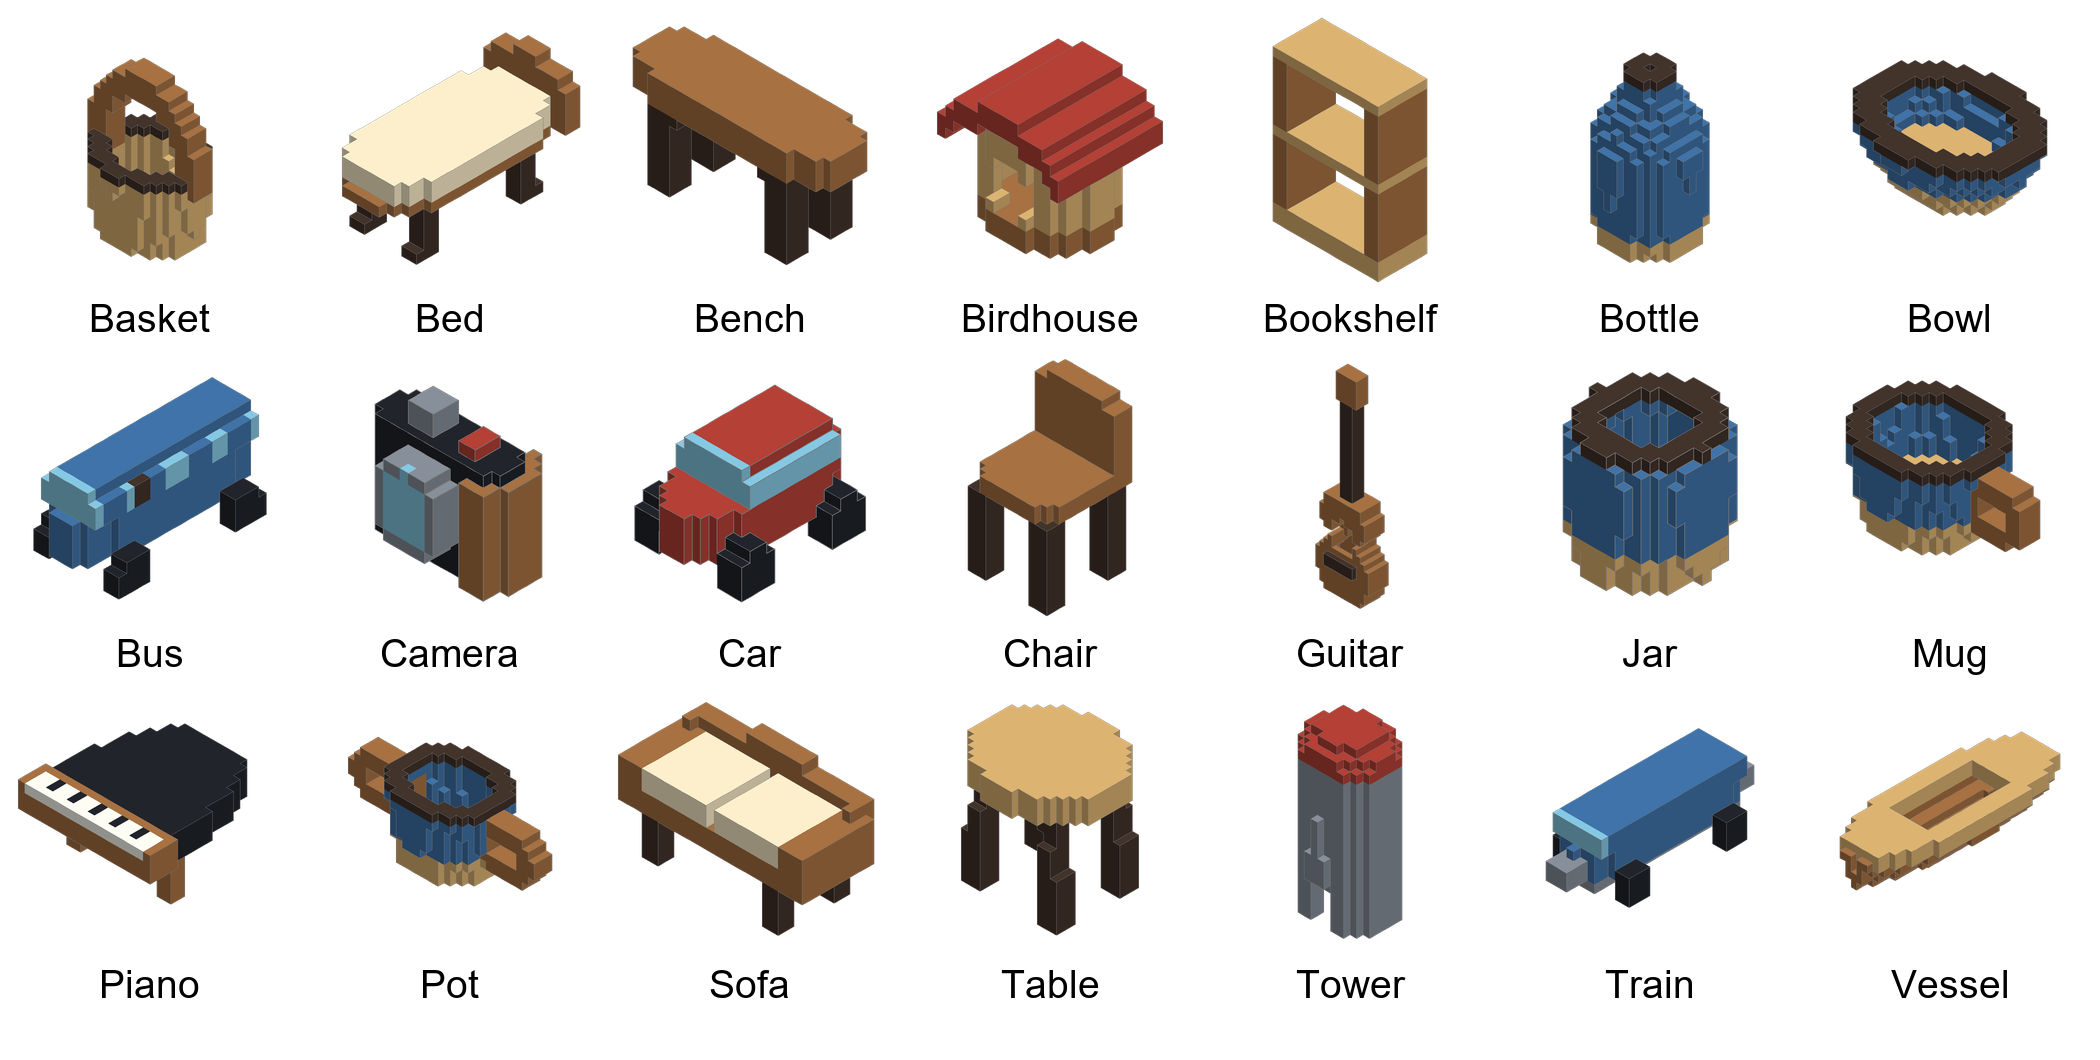
\includegraphics[width=\textwidth]{figures/image7_en.png}
\caption{Voxel model samples spanning the 21 object categories.}
\end{figure*}

\begin{figure*}[t]
\centering
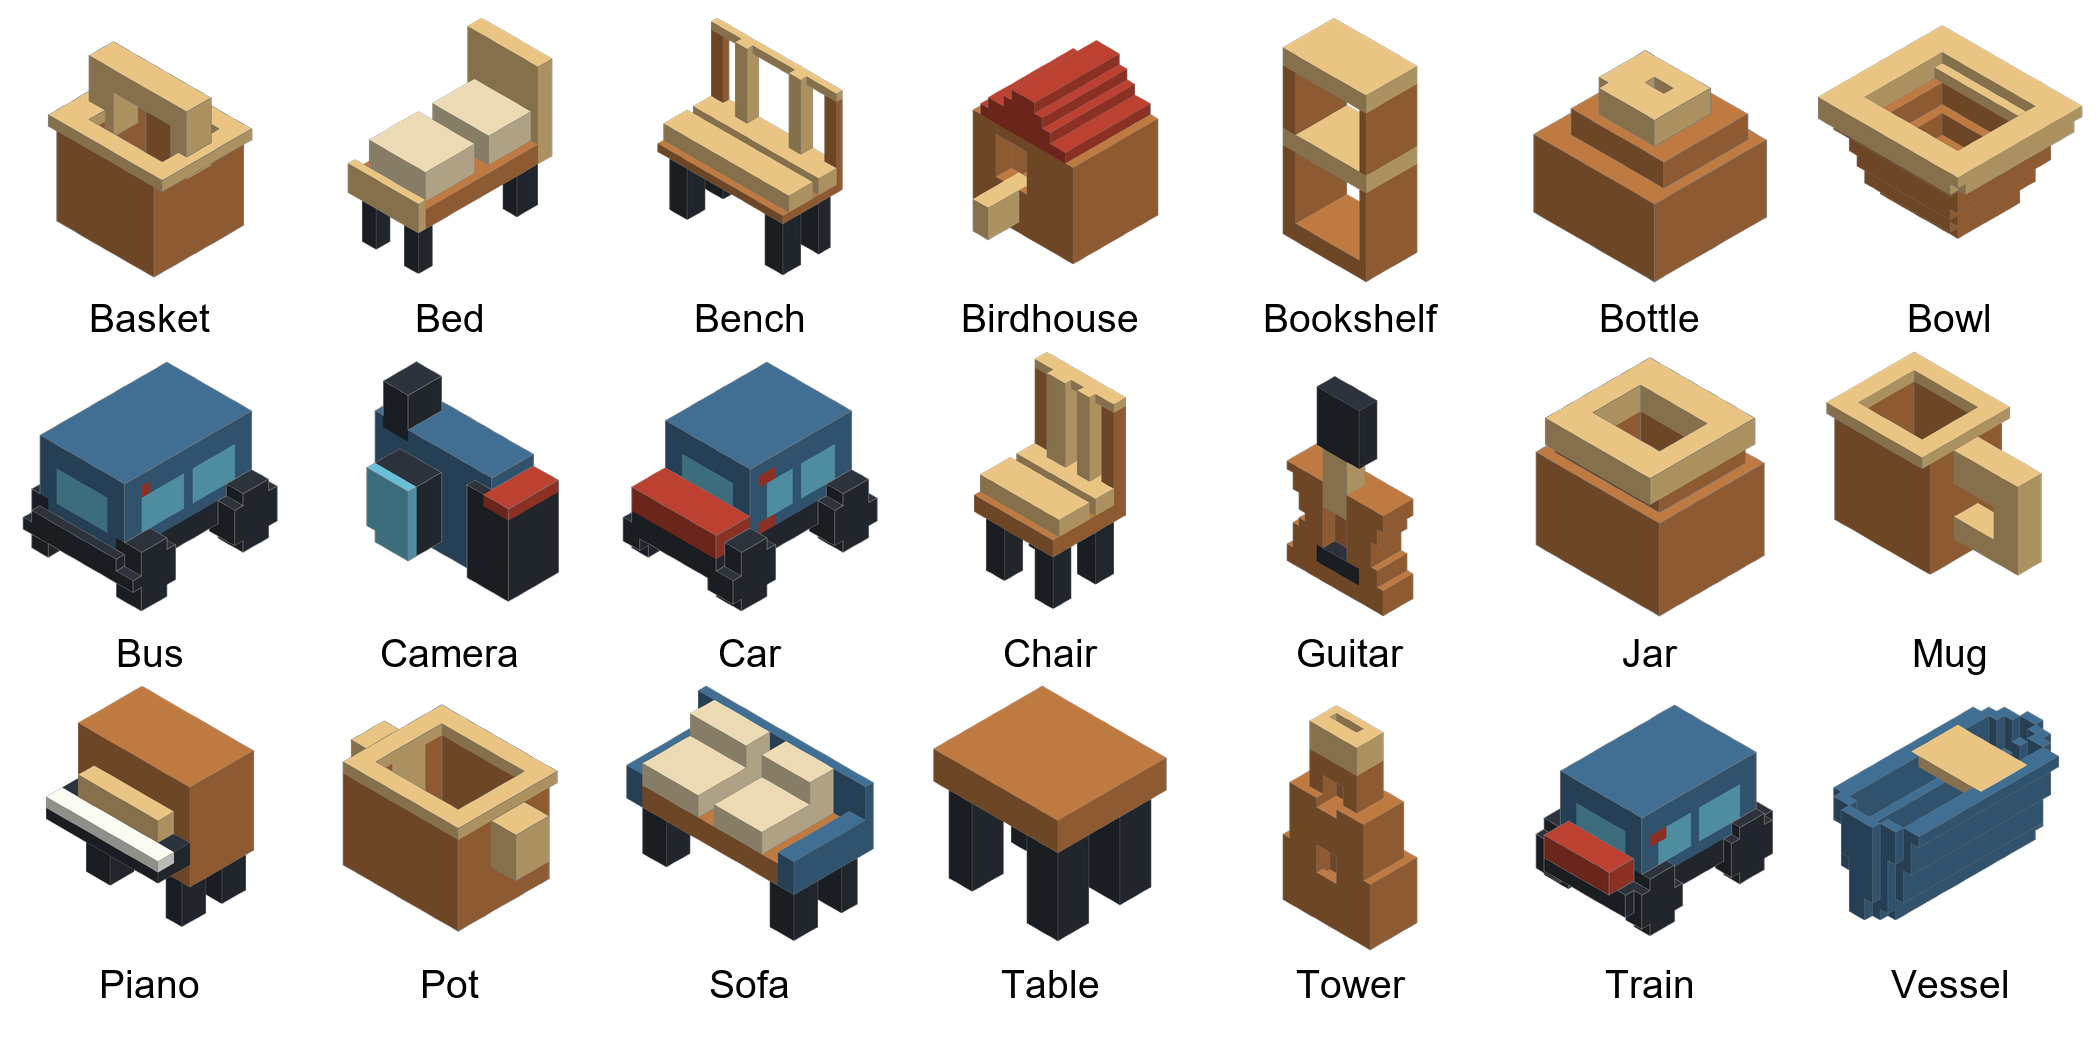
\includegraphics[width=\textwidth]{figures/image8_en.png}
\caption{Additional historical voxel model examples.}
\end{figure*}

\begin{figure*}[!htbp]
\centering
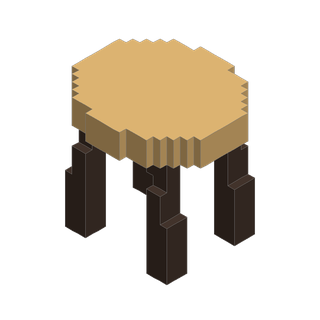
\includegraphics[width=0.118\textwidth]{figures/image4.png}\hfill
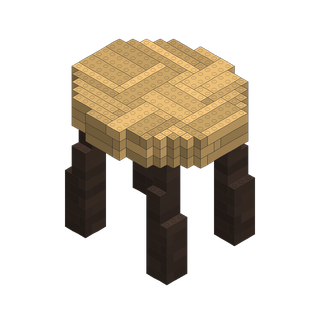
\includegraphics[width=0.118\textwidth]{figures/image5.png}\hfill
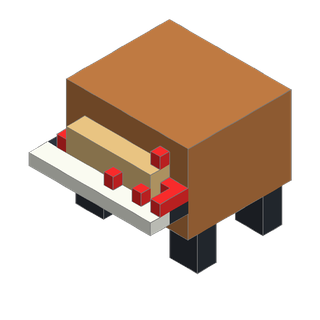
\includegraphics[width=0.118\textwidth]{figures/image2.png}\hfill
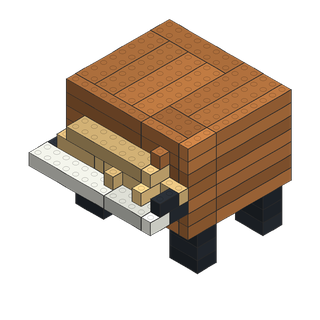
\includegraphics[width=0.118\textwidth]{figures/image3.png}\hfill
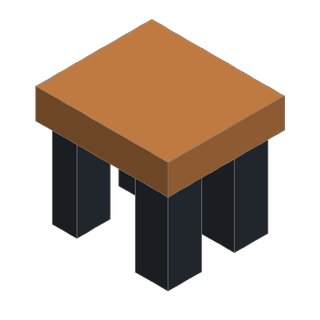
\includegraphics[width=0.118\textwidth]{figures/image9.png}\hfill
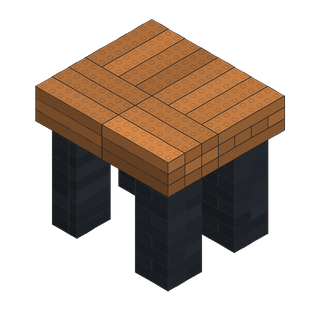
\includegraphics[width=0.118\textwidth]{figures/image10.png}\hfill
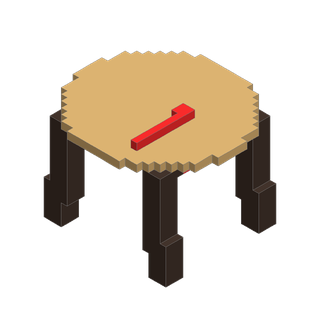
\includegraphics[width=0.118\textwidth]{figures/image11.png}\hfill
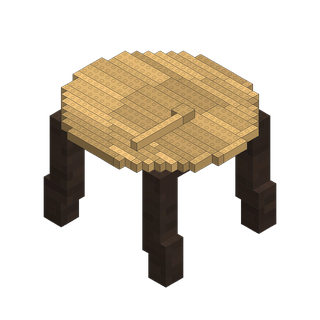
\includegraphics[width=0.118\textwidth]{figures/image12.png}
\caption{Historical examples of voxel targets and brick layouts after local repair.}
\end{figure*}

\begin{figure*}[t]
\centering
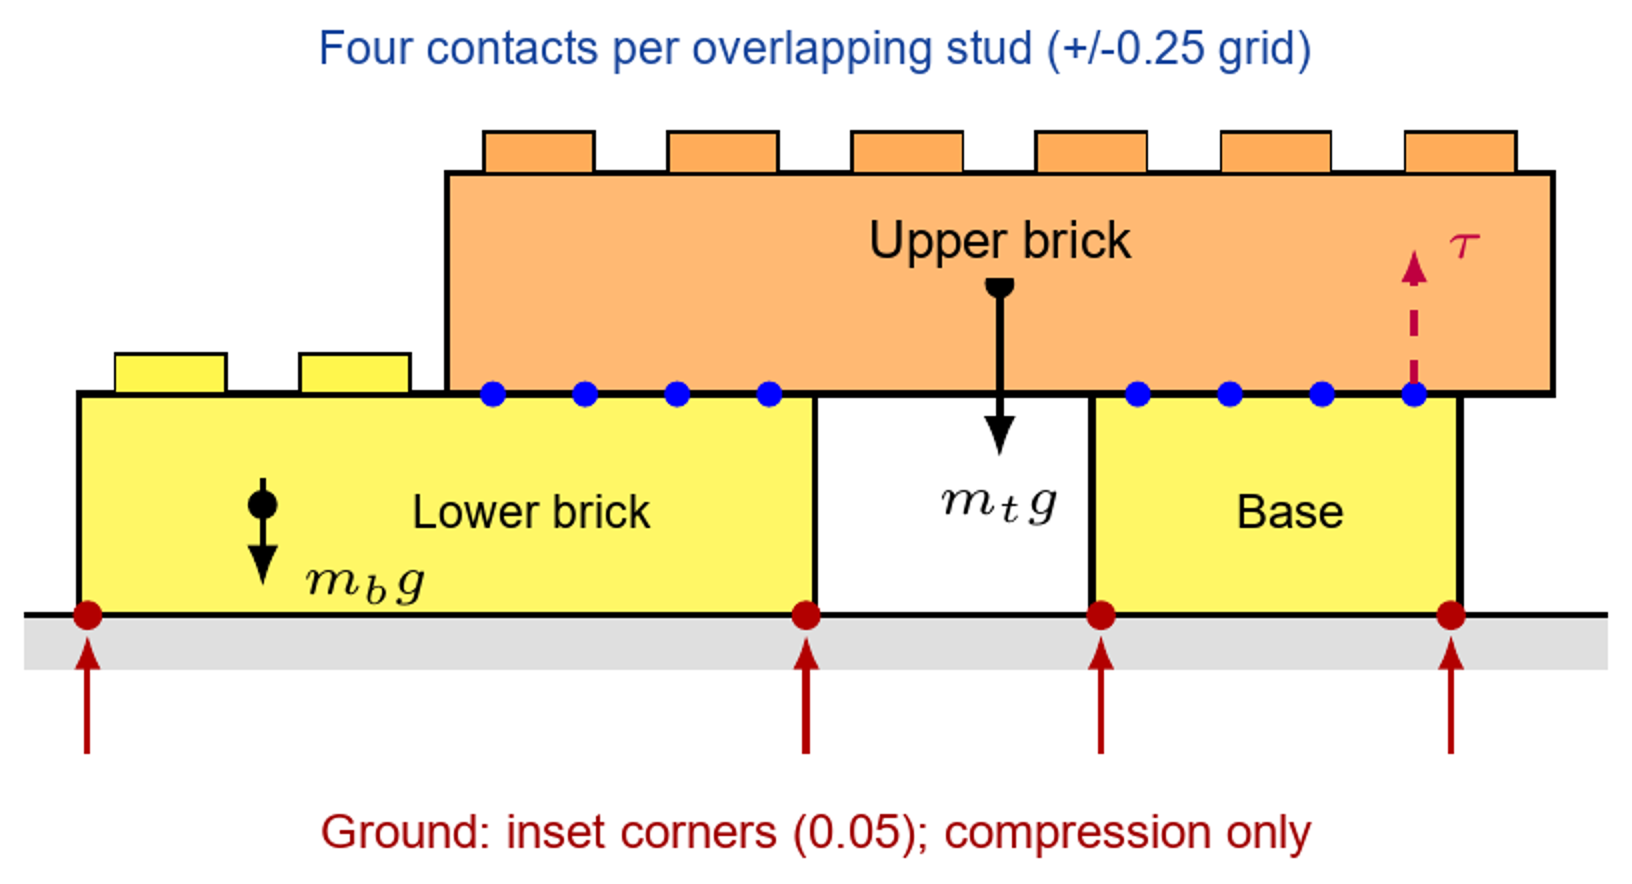
\includegraphics[width=0.75\textwidth]{figures/image13_en.png}
\caption{Historical contact-based gravity screening model, with English labels. The stated contact and ground assumptions are retained.}
\end{figure*}

\begin{figure*}[!htbp]
\centering
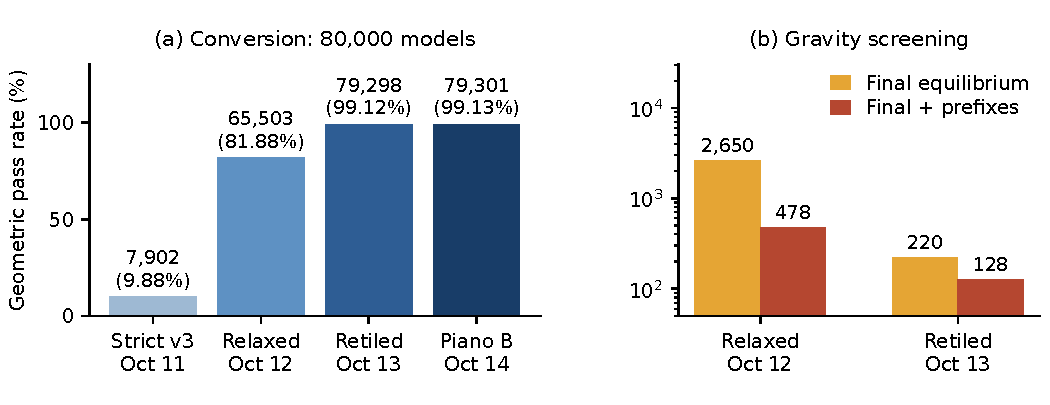
\includegraphics[width=\textwidth]{figures/image14_en.pdf}
\caption{Historical comparison of geometric conversion and screening outcomes across releases; values as in the corresponding release reports (Table~\ref{tab:conversion}).}
\end{figure*}

\begin{figure*}[!htbp]
\centering
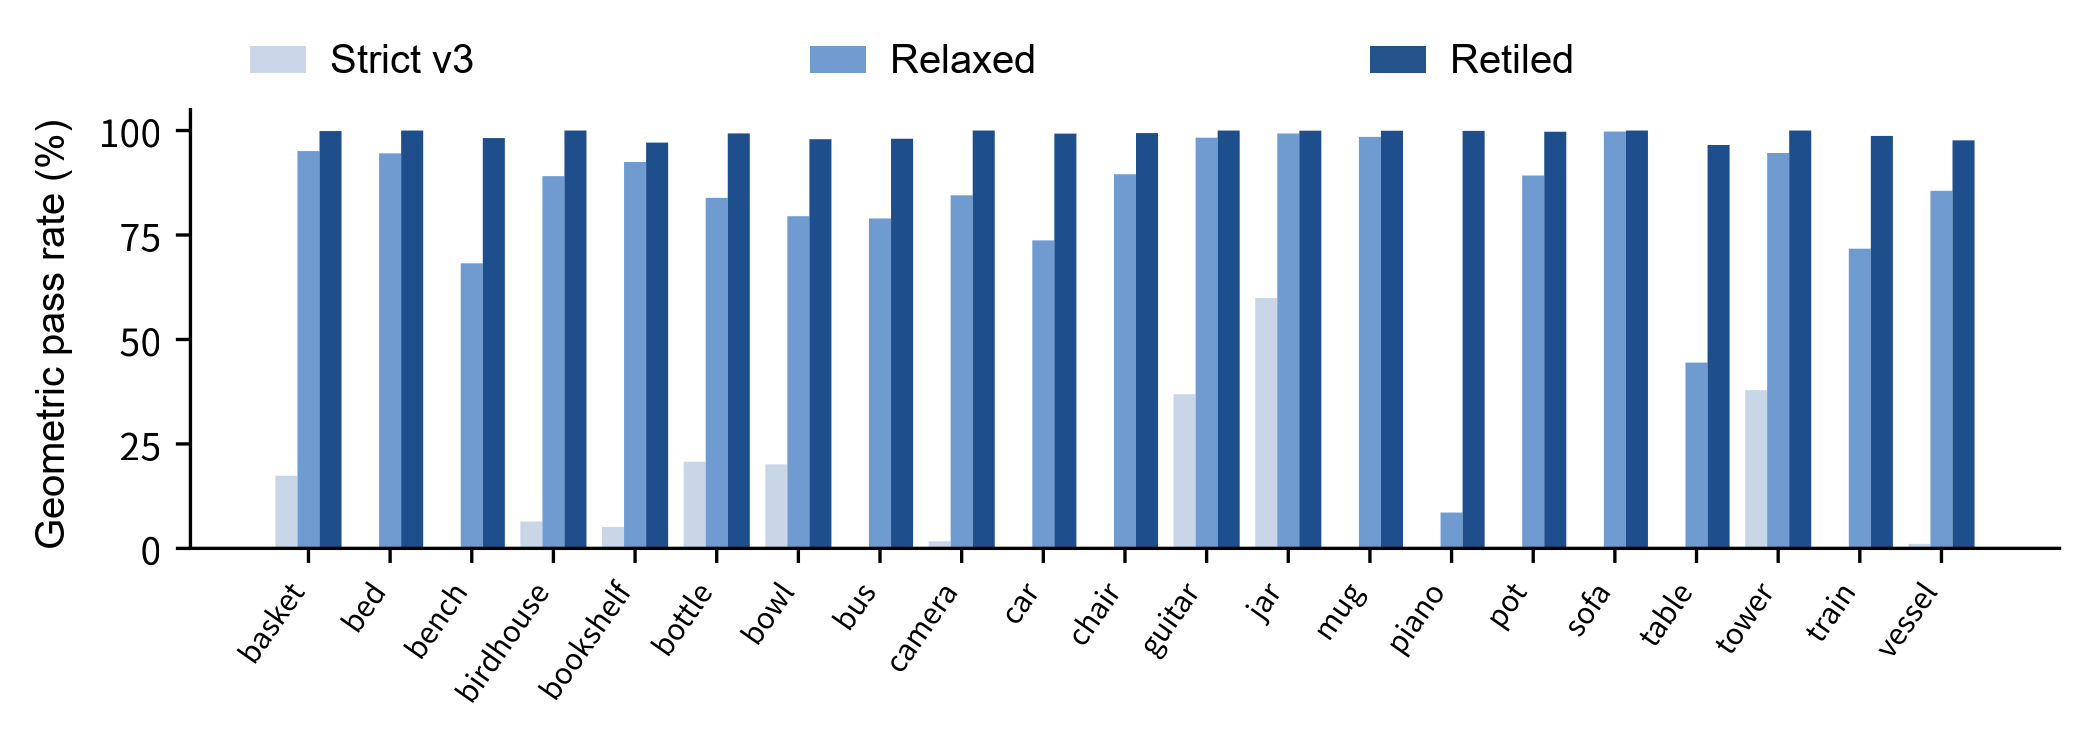
\includegraphics[width=\textwidth]{figures/image15_en.png}
\caption{Historical category-level geometric pass rates. Version and numerical labels require verification.}
\end{figure*}

\begin{figure*}[t]
\centering
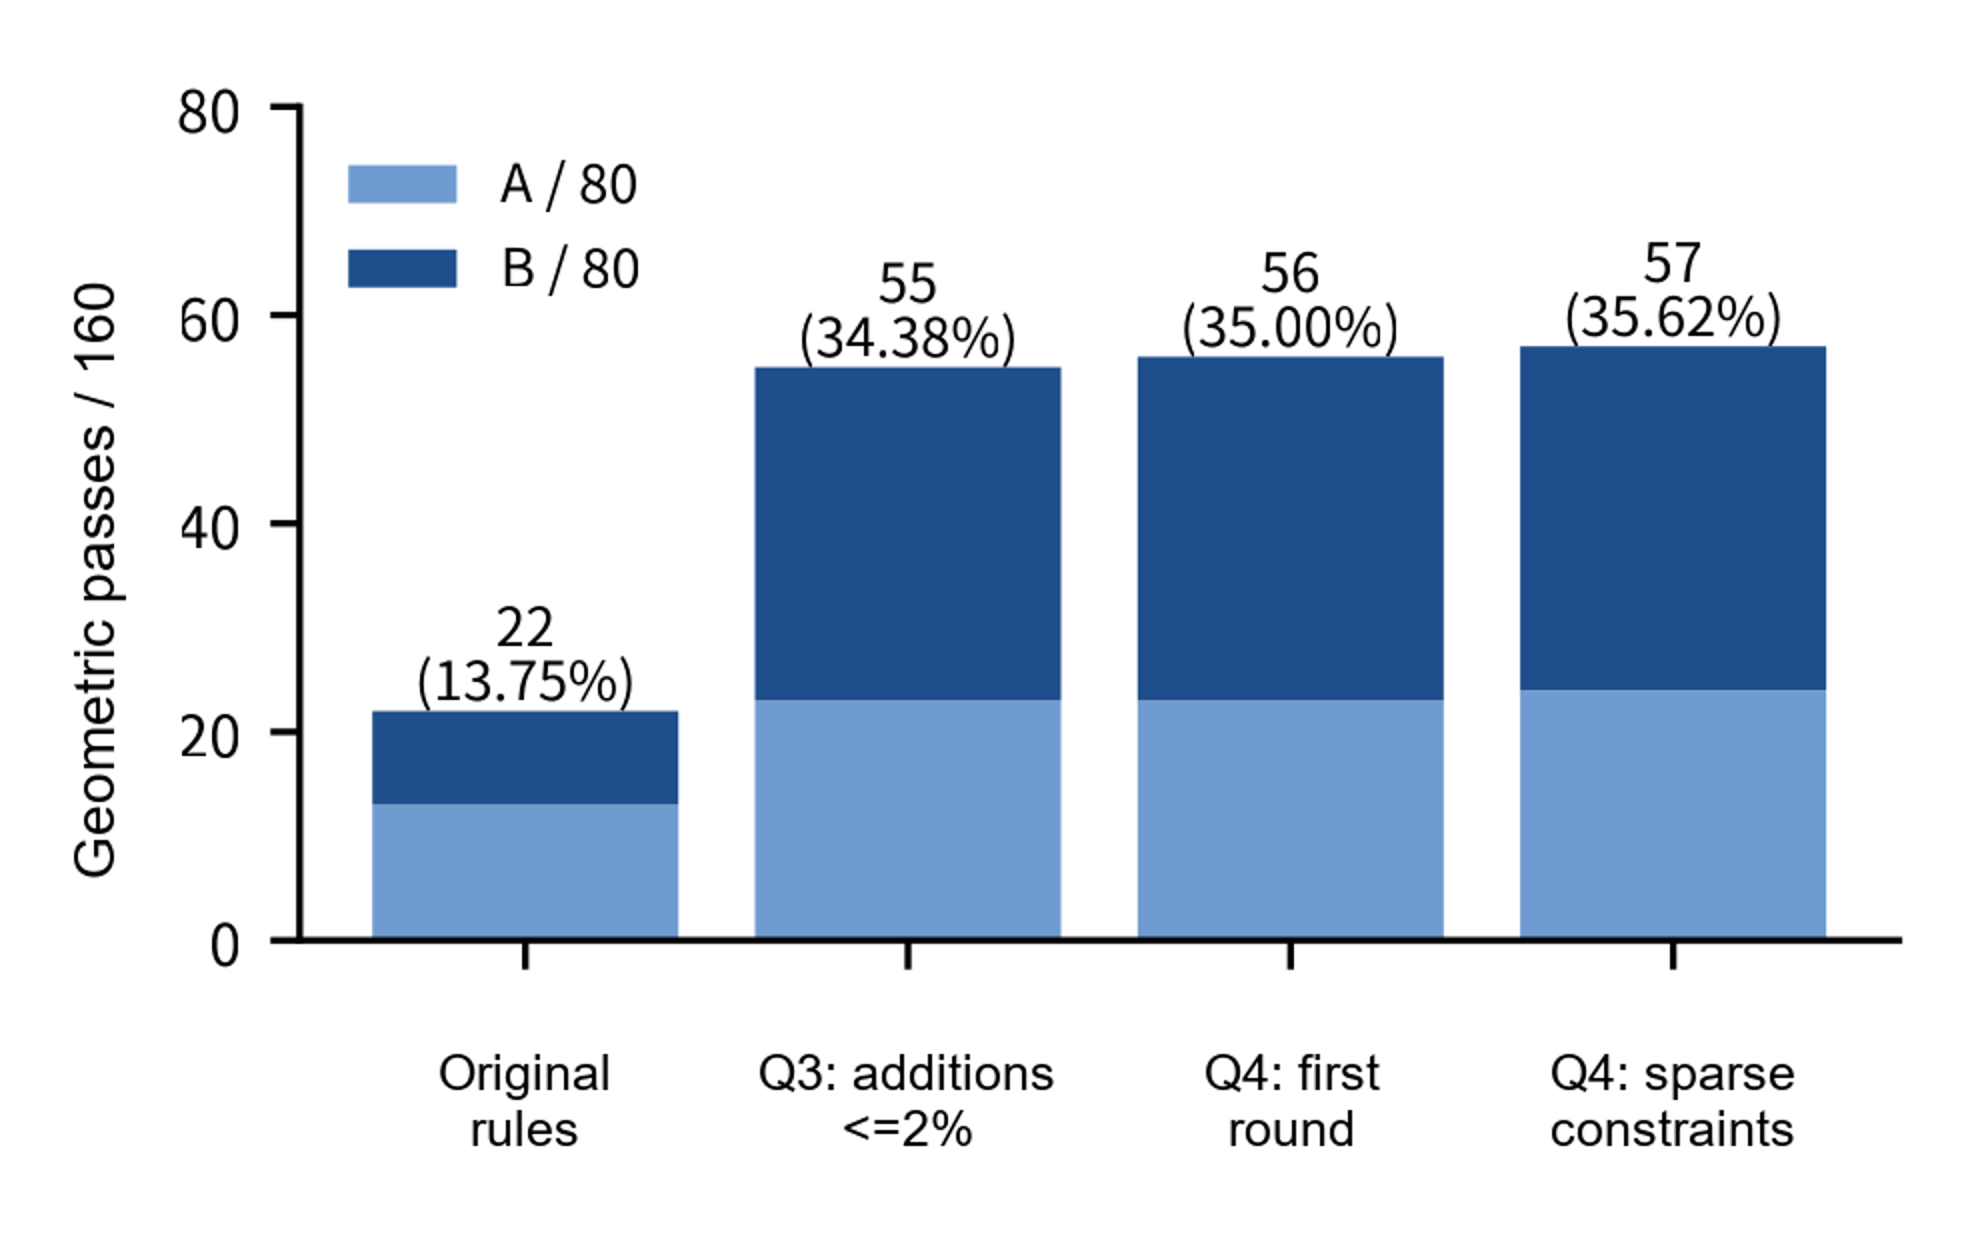
\includegraphics[width=0.72\textwidth]{figures/image16_en.png}
\caption{Historical results on a uniform 160-model sample. Version and numerical labels require verification.}
\end{figure*}

\begin{figure*}[!htbp]
\centering
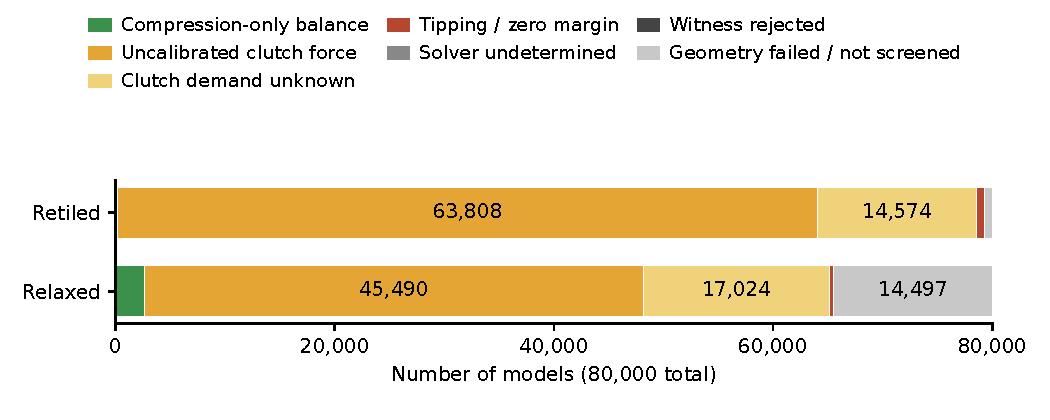
\includegraphics[width=\textwidth]{figures/image17_en.pdf}
\caption{Historical distributions of physical screening statuses; values as in the corresponding release reports. Counts refer to the specific releases shown and are kept separate from geometric pass rates.}
\end{figure*}


\section{Technical Appendix: Training Details}
\label{app:training}
Aggregate throughput is 24,448 tokens/s over eight GPUs, and the mean training loss is 0.0273. Evaluation and checkpointing run every 500 steps. With TRL~0.15, the unpacked multi-GPU path hangs after the first backward pass, which is why the TRL~0.17 stack is pinned. Because validation loss is lowest during epoch 2, two epochs would be a more economical setting for future runs (about one third less compute). The full software stack is transformers 4.51.3, trl 0.17.0, peft 0.15.2, datasets 3.6.0, and accelerate 1.6.0, with bf16 precision, gradient checkpointing, and unpacked sequences.

\begin{table}[!htbp]
\centering
\small
\begin{tabular}{lrr}
\toprule
Progress & Step & Validation loss \\
\midrule
Start & 500 & 0.1410 \\
--- & 1,500 & 0.0950 \\
--- & 10,500 & 0.0509 \\
--- & 22,500 & 0.0404 \\
$\approx$ End of epoch 1 & 44,500 & 0.0337 \\
--- & 65,500 & 0.0316 \\
Best (epoch 1.77) & 79,000 & 0.0308 \\
End of epoch 3 & 133,860 & 0.0339 \\
\bottomrule
\end{tabular}
\caption{Validation loss on the 2,000-sample validation subset. One epoch is $\approx$44,620 steps; the nearest evaluation to the end of epoch 1 is step 44,500.}
\label{tab:eval-loss}
\end{table}

% BrickGPT-paper column verified against arXiv:2505.05469 (Sec. 5.1 and Appendix A training details).
\begin{table*}[!htbp]
\centering
\small
\setlength{\tabcolsep}{5pt}
\begin{tabular}{lcc}
\toprule
Dimension & BrickGPT paper & Official Qwen3 script (ours) \\
\midrule
Base model & LLaMA-3.2-1B-Instruct & Qwen3-1.7B \\
LoRA & $r=32$, $\alpha=16$, dropout $0.05$, $q$/$v$ only (3.4M params) & $r=16$, $\alpha=32$, all linear layers \\
Learning rate & $2{\times}10^{-3}$ (AdamW) & $10^{-4}$ \\
Effective batch & 64 & 8 \\
Max length & 4,096 & 8,192 \\
Epochs & 3 & 3 \\
Hardware & 8$\times$RTX A6000, 12\,h & 8$\times$4090D, 25.3\,h \\
Data & StableText2Brick, 47k structures / 240k prompts & BrickMore-48, 79.3k models / 396,610 samples \\
\bottomrule
\end{tabular}
\caption{Our configuration versus the original BrickGPT paper \cite{brickgpt}. BrickGPT-paper values are taken from Sec.~5.1 and Appendix~A of arXiv:2505.05469 (base model, LoRA $r{=}32$, $\alpha{=}16$, dropout $0.05$, $q$/$v$ only with 3.4M parameters, AdamW learning rate $0.002$, global batch 64, 4096-token length filter, 3 epochs, 8$\times$RTX A6000 and 12\,h, and 47k+ structures / 240k prompts). The data organization, instruction template, absence of thinking mode, and LoRA paradigm follow BrickGPT; concrete hyperparameters follow the official Qwen3 adaptation, with the budget adjusted for the larger world, library, and corpus.}
\label{tab:brickgpt-recipe}
\end{table*}


\section{Technical Appendix: Additional Evaluation Material}
\label{app:eval}

\paragraph{November 16 evaluation.}
The run processed 1,315 exports and 10,520 images, with all four metrics present for each export. Group B contains 265 raw BrickForma Q8\_0 exports, 265 BrickGPT exports, and 265 BrickNet exports. The BrickGPT records report a $20^3$ world, seed 42, an eight-regeneration budget, and Gurobi disabled. Group A supplies only BrickGPT and BrickNet, with 260 exports per system (Table~\ref{tab:group-a}). The Group A BrickGPT run used the official merged checkpoint, a $20^3$ world, seed 42, and a 100-regeneration budget. Baseline means are reported within each cohort because the prompts and BrickGPT settings differ.
\begin{table}[t]
\centering\small
\setlength{\tabcolsep}{3pt}
\begin{tabular}{lrrrr}
\toprule
System & $P_{\mathrm{inv}}\downarrow$ & VQAScore $\uparrow$ & PE $\uparrow$ & SigLIP2 $\uparrow$ \\
\midrule
BrickGPT & \textbf{0.00\%} & \textbf{0.0401} & \textbf{0.1422} & \textbf{0.0125} \\
BrickNet & 18.97\% & 0.0142 & 0.1201 & 0.0007 \\
\bottomrule
\end{tabular}
\caption{Group A means on 260 matched prompts. This cohort contains BrickGPT and BrickNet.}
\label{tab:group-a}
\end{table}


\paragraph{Paired tests and truncation.}
Table~\ref{tab:sig} compares Group B alignment scores by prompt. We use a two-sided exact sign test and a two-sided Wilcoxon signed-rank test with the normal approximation, excluding ties from each test. Holm correction is applied separately to the six comparisons within each test. The largest adjusted $p$ is $4.62{\times}10^{-5}$ (rounded up). PE truncates 59 of 265 prompts and SigLIP2 truncates 106. On the untruncated subsets, BrickForma / BrickGPT / BrickNet score 0.1519 / 0.1430 / 0.1116 on PE (206 prompts) and 0.0404 / 0.0179 / 0.0009 on SigLIP2 (159 prompts).
\begin{table}[t]
\centering\small
\setlength{\tabcolsep}{3pt}
\begin{tabular}{llrrr}
\toprule
Baseline & Metric & W/L/T & Sign $p_H$ & Wilc.\ $p_H$ \\
\midrule
BrickGPT & VQAScore & 188/77/0 & $2.1\times 10^{-11}$ & $3.0\times 10^{-8}$ \\
 & PE & 166/99/0 & $4.6\times 10^{-5}$ & $3.8\times 10^{-6}$ \\
 & SigLIP2 & 168/97/0 & $3.1\times 10^{-5}$ & $2.2\times 10^{-6}$ \\
BrickNet & VQAScore & 237/28/0 & $1.2\times 10^{-41}$ & $5.9\times 10^{-33}$ \\
 & PE & 209/56/0 & $3.1\times 10^{-21}$ & $3.0\times 10^{-25}$ \\
 & SigLIP2 & 207/57/1 & $1.4\times 10^{-20}$ & $8.1\times 10^{-24}$ \\
\bottomrule
\end{tabular}
\caption{Two-sided paired tests on Group B. W/L/T counts BrickForma wins, losses and ties. Each test uses Holm correction across six comparisons.}
\label{tab:sig}
\end{table}


\paragraph{Earlier 114-prompt comparison.} BrickGPT outputs were generated in its native $20^3$ world (seed 42), whereas BrickForma places bricks in a $48^3$ workspace, which partly explains the difference in part counts.
The systems differ in candidate selection, filtering, and post-processing.
On the BrickForma side, 45 of the 114 comparison outputs, together with their prompts, were chosen by human review as the best of six candidate phrasings in a category--level group; a winner was available in 79 of 105 groups, and 45 of those winners entered this comparison.
The remaining 69 outputs come from later fill-in, regeneration, colleague, and review rounds: 35 replaced a judged winner in 34 groups, and 34 filled 26 groups in which no candidate had been judged acceptable; together the 114 outputs cover all 105 groups.\footnote{The six candidates are the five new-batch phrasings and one first-batch phrasing documented in the evaluation-set README. Among the 69: \texttt{review\_59} 21, a colleague success set 16, second-round redo 12, third-round fill-in 7, colleague \texttt{nine\_ldr} 7, regeneration 5, and \texttt{car\_trials} 1, as recorded in the 11-07 delivery manifest. BrickGPT was then run once on each selected prompt (seed 42); BrickNet contributed one accepted sample per prompt (up to 30 attempts).}
The 114 outcomes comprised 110 retiled layouts and four raw layouts. The earlier BrickGPT records report an eight-regeneration budget and Gurobi disabled.

\paragraph{Sensitivity of the earlier comparison.}
With equal weighting over the 105 category--level groups, BrickForma scores 0.2347 / 0.1840 / 0.1257 and BrickGPT scores 0.1511 / 0.1459 / 0.0318 on VQAScore / PE / SigLIP2. After excluding prompts truncated by each encoder, PE is 0.1821 versus 0.1445 on 89 prompts and SigLIP2 is 0.1088 versus 0.0301 on 85 prompts. The PE and SigLIP2 text encoders read at most 72 and 64 tokens, respectively.

\paragraph{Diagnostic cohort.}
To probe what the fine-tuned model learns, we inspected 525 BrickForma generations from a diagnostic set (21 categories $\times$ five levels $\times$ five phrasings). The 525-prompt diagnostic batch, together with 105 first-batch prompts, formed the six-phrasing candidate pool from which 45 of the 114 comparison outputs were selected (35 of them from the 525), as described above. Generation used seeds 42, 104, and 2026 in that order, moving to the next seed when a draft was incomplete or failed the geometry validator, then applied the 12--60--180\,s MILP ladder (the default loop of Algorithm~\ref{alg:inference-retiling}); raw drafts that already formed a single stud-connected component were kept unchanged. For 28 prompts a recovery path sampled seeds outside $S$; for two further prompts the solver budget was extended to 600\,s. Only 46 raw layouts (8.8\%) form a single stud-connected component without retiling; this rate shows no clear trend across levels (13, 9, 9, 7, and 8 for L1--L5) but varies strongly by category (e.g., 8/25 for sofa, 0/25 for basket and camera). All 479 failing raw layouts split into at least two stud components (median 5, maximum 33). Overlaps are a minor cause: 50 failing layouts contain duplicated voxels, 41 of them with at most five (median 2), and 429 contain none. The 2,240 detached fragments are mostly not grounded (1,320 airborne versus 920 grounded). The learned representation thus places bricks whose in-bounds voxel union is retained by retiling but that often fail to interlock across layers; all 525 final assemblies form a single stud-connected component with that union unchanged (Table~\ref{tab:diag} in Appendix~\ref{app:eval}). These checks evaluate stud connectivity and in-bounds voxel-union consistency, not prompt-level shape fidelity or spatial reasoning.

\begin{table}[t]
\centering
\small
\begin{tabular}{lrr}
\toprule
Metric & Raw & Retiled \\
\midrule
$P_{\mathrm{inv}}$ $\downarrow$ & 0.1897\% & 0.0000\% \\
VQAScore $\uparrow$ & 0.2065 & 0.2071 \\
PE $\uparrow$ & 0.1858 & 0.1859 \\
SigLIP2 $\uparrow$ & 0.1379 & 0.1261 \\
Mean parts & 178.7 & 421.2 \\
\bottomrule
\end{tabular}
\caption{Earlier repair comparison on 110 pairs sharing the same prompt, model identifier, and caption.}
\label{tab:raw-retiled}
\end{table}

\begin{figure*}[t]
\centering
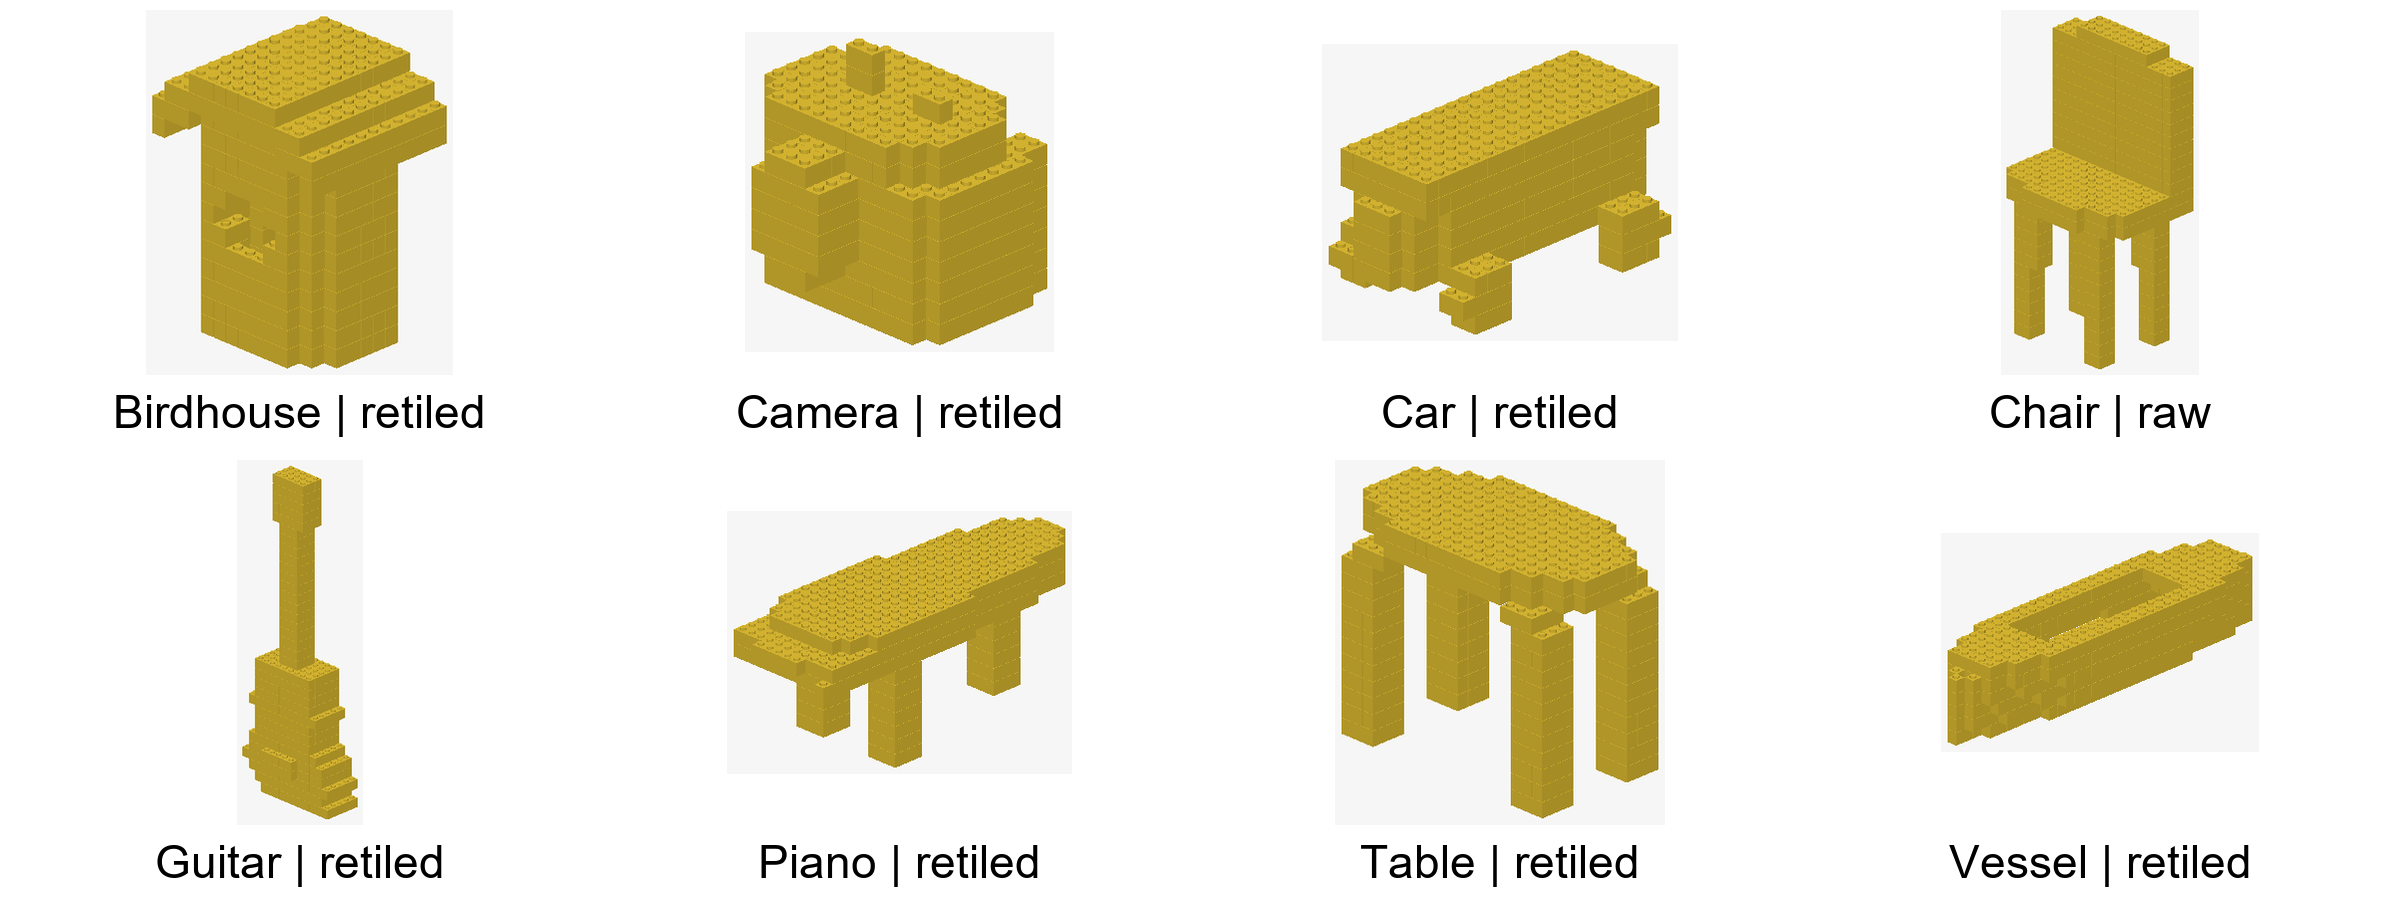
\includegraphics[width=\textwidth]{figures/generated_gallery_en.png}
\caption{BrickForma outputs from the earlier 114-prompt comparison. The chair is raw and the remaining examples are retiled.}
\end{figure*}


\begin{table*}[!htbp]
\centering
\small
\setlength{\tabcolsep}{3pt}
\begin{tabular}{lr}
\toprule
Quantity (525 prompts) & Value \\
\midrule
Raw layout is a single stud component & 46 (8.8\%) \\
Stud components per failing raw (med./max) & 5 / 33 \\
Failing raw layouts with duplicated voxels & 50 / 479 \\
Detached fragments (airborne / grounded) & 1,320 / 920 \\
MILP tier reached (12 / 60 / 180 / 600\,s) & 326 / 133 / 18 / 2 \\
Prompts resampled outside $S$ & 28 \\
Final: single stud comp., union unchanged & 525 / 525 \\
Raw bricks, median (range) & 183 (77--623) \\
Final assembly bricks, median & 452 \\
\bottomrule
\end{tabular}
\caption{Structural diagnostics of raw outputs (Section~\ref{sec:diagnostics}). ``Union unchanged'' means the final assembly covers exactly the in-bounds voxel union of the raw draft; it does not assess whether the shape matches the prompt.}
\label{tab:diag}
\end{table*}



\begin{figure*}[!htbp]
\centering
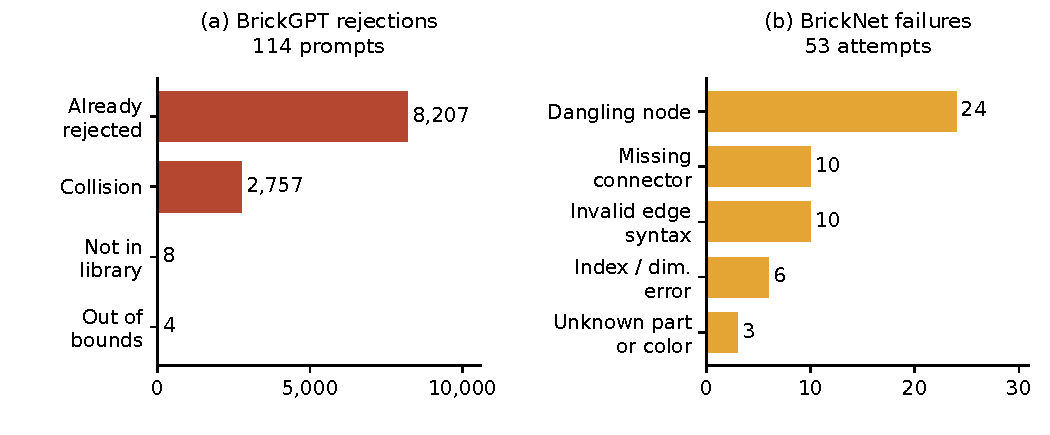
\includegraphics[width=\textwidth]{figures/image19_en.pdf}
\caption{Historical failure categories in the supplied reference; values as in the corresponding run records.}
\end{figure*}

\begin{figure*}[!htbp]
\centering
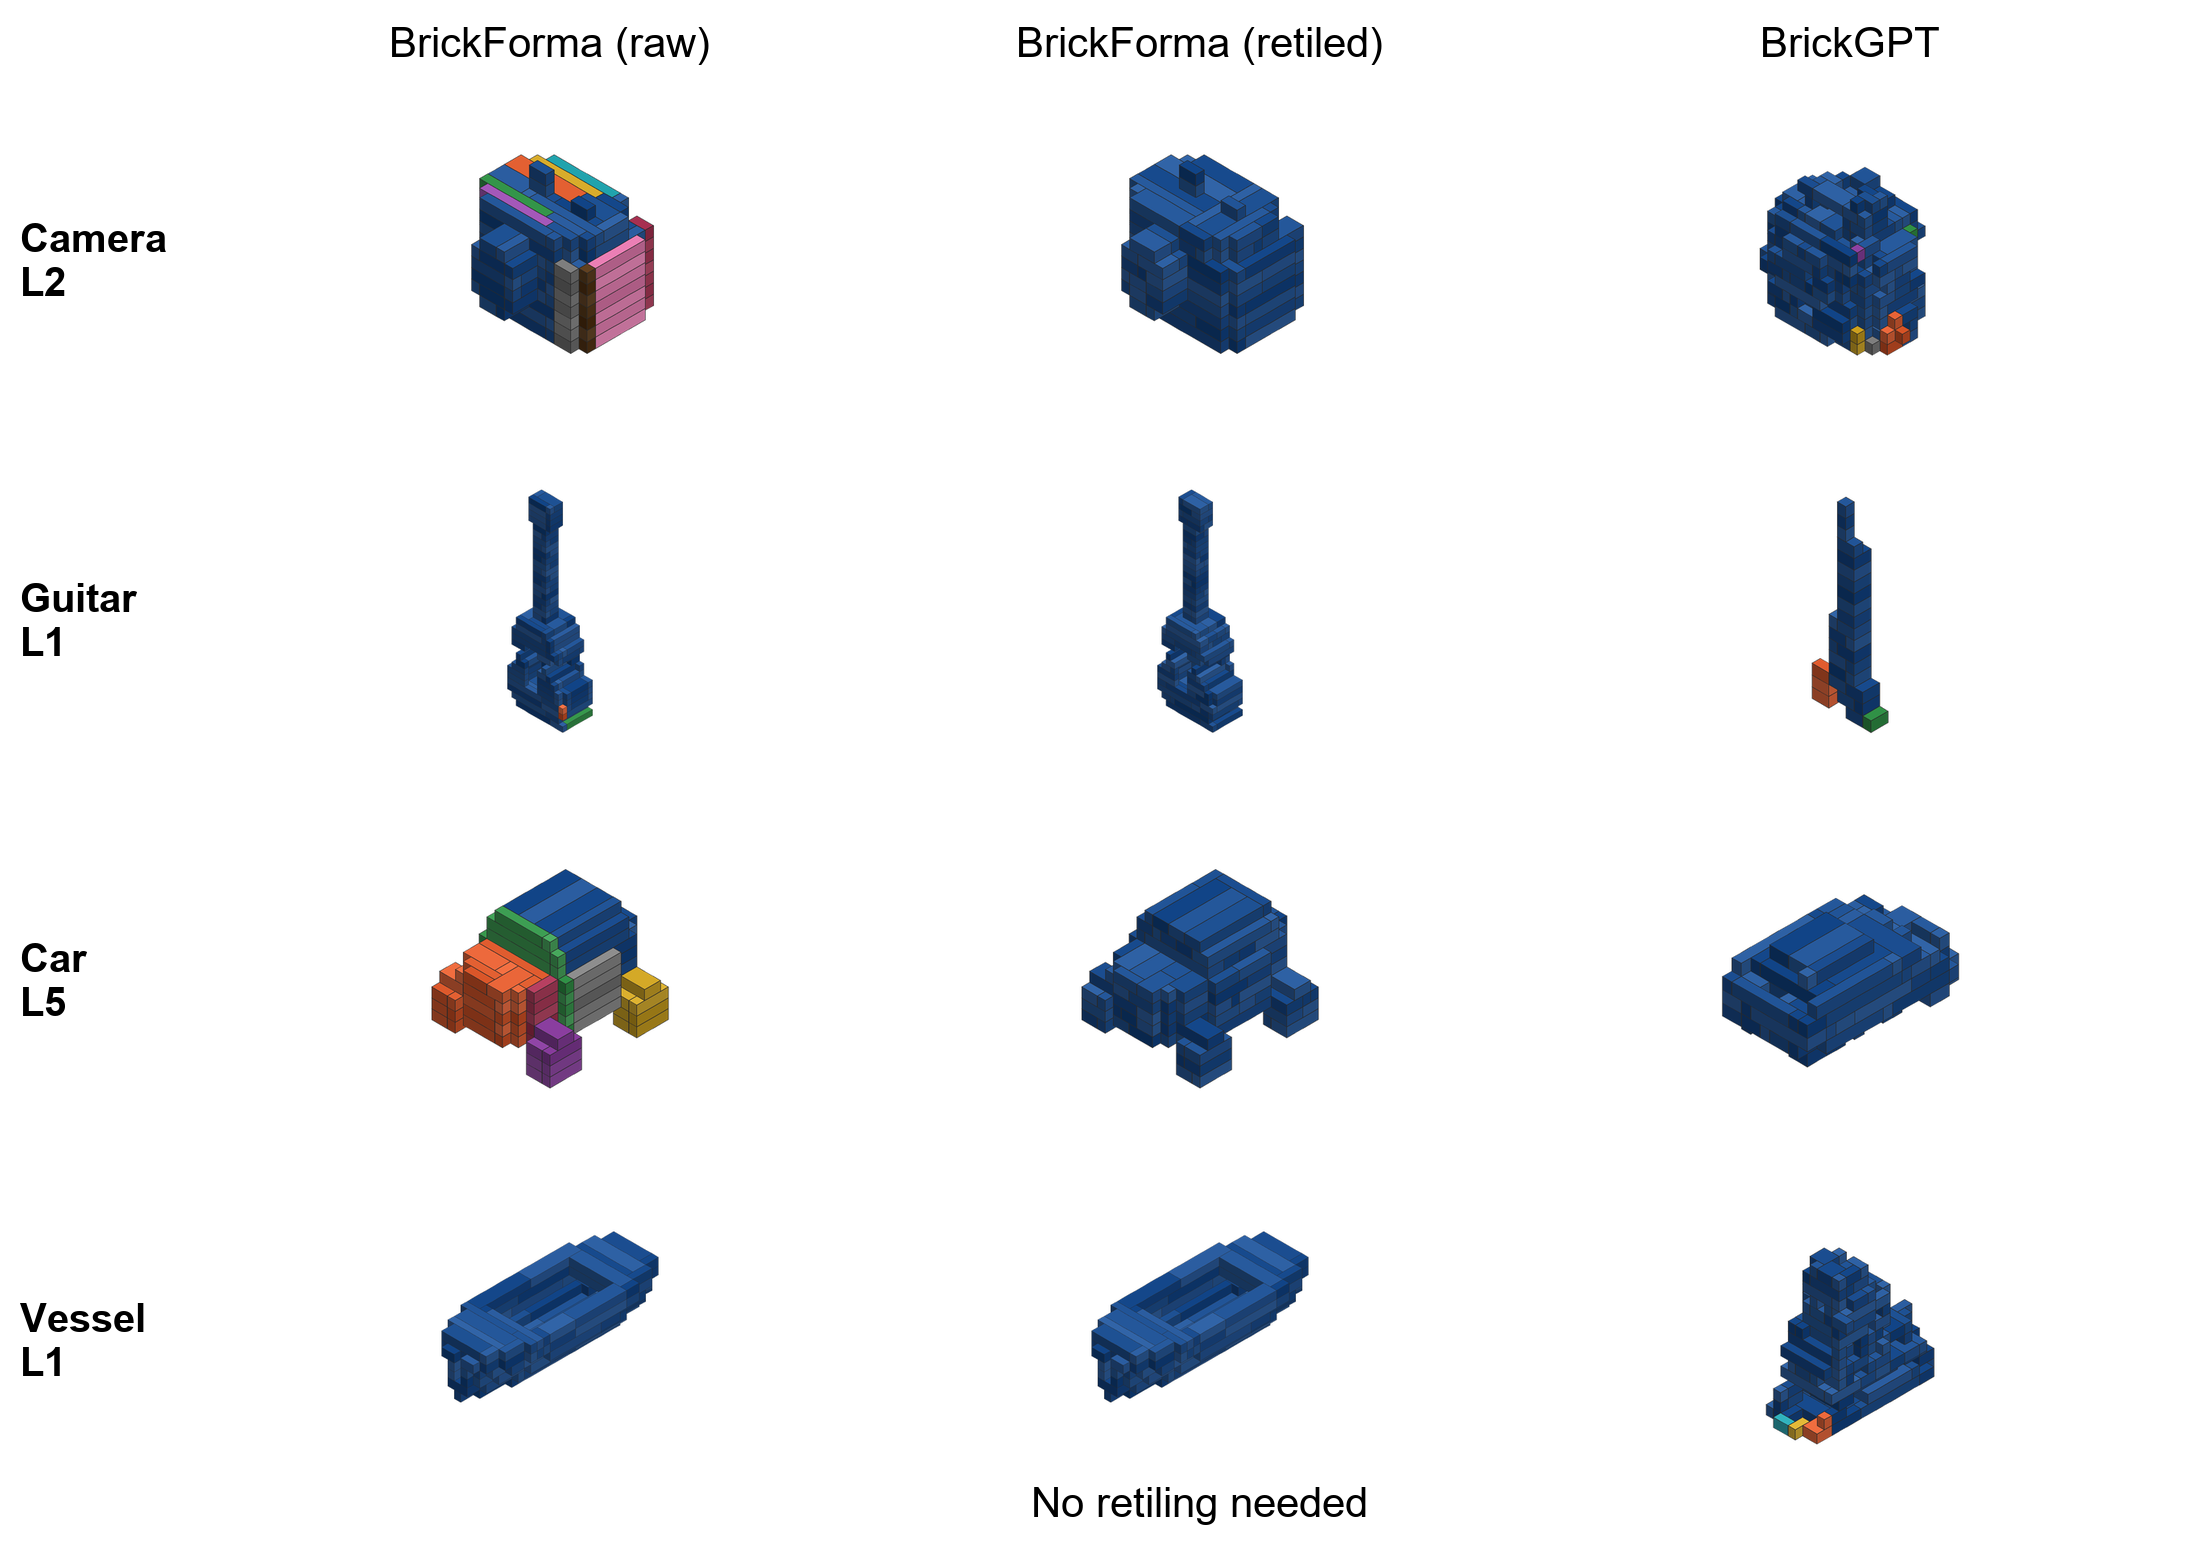
\includegraphics[width=\textwidth]{figures/original_comparison_en.png}
\caption{Qualitative historical examples from the supplied reference. Columns show raw and retiled outputs of our system and BrickGPT outputs.}
\end{figure*}


\section{Technical Appendix: Historical Tables}
\label{app:historical}
The following transcribed tables preserve the historical reference material. They use different versions or evaluation criteria and are not substitutes for the current main comparison. Where a value is superseded by a verified number in the main text (e.g., Table~\ref{tab:training-data} and Appendix~\ref{app:dataset}), the main text takes precedence. Dashes indicate missing entries in the supplied source.
\begin{table*}[!htbp]\centering\small
\begin{tabular}{lr}\toprule
Item & Historical value \\ \midrule
Voxel models & 80,000 (40,000 per batch) \\
Categories / structural families & 21 / 40 per category \\
Grid / voxel count & $48^3$ / 750--1,250 \\
Prompt records & 400,000 (five bilingual records per model) \\
Uniqueness & 80,000 unique; 0 A/B duplicates \\
Overlap with historical hashes & 0 / 55,255 \\
Retile geometry passes & 79,298 (99.12\%) \\
Bricks in full preview & 12,718,389 \\
Final gravity equilibrium passes & 220 \\
Final and layer-prefix passes & 128 \\
\bottomrule\end{tabular}
\caption{Historical dataset statistics transcribed from the supplied reference. The geometry count refers to the old retile release, not the later integrated count. Verify the preview and physical-screening totals against version-matched reports.}
\end{table*}

\begin{table*}[!htbp]\centering\small
\setlength{\tabcolsep}{3pt}
\begin{tabular}{@{}l>{\raggedright\arraybackslash}p{3.9cm}>{\raggedright\arraybackslash}p{2.5cm}rrrr@{}}\toprule
Version & Connectivity & Voxel changes & Passes & Rate & Final & Both \\ \midrule
Strict v3 & Single; support $\geq$10\%, overhang $\leq$2 & None & 7,902 & 9.88\% & -- & -- \\
Relaxed & Each component grounded & +428,278 / -38,230 & 65,503 & 81.88\% & 2,650 & 478 \\
Retile & Each component grounded & +228,582 / -125 & 79,298 & 99.12\% & 220 & 128 \\
\midrule
\multicolumn{7}{l}{Uniform 160-model sample (seed 38177); not full-dataset results} \\
Baseline & Single stud-connected component & None & 22 & 13.75\% & -- & -- \\
Q3 & Single stud-connected component & Added $\leq$2\% & 55 & 34.38\% & 8 & 2 \\
Q4 (sparse) & Single stud-connected component & Added + removed $\leq$2\% & 57 & 35.63\% & 8 & 2 \\
\bottomrule\end{tabular}
\caption{Historical conversion-strategy table from the reference. Full-dataset and 160-model sample rows use different scopes; connectivity rules also differ. Final and Both columns report final-equilibrium and final-plus-prefix screening passes under the stated historical assumptions.}
\end{table*}

\begin{table*}[!htbp]\centering\small
\begin{tabular}{lrrr}\toprule
Item & BrickGPT & BrickNet 1.7B & BrickMore-48 \\ \midrule
Representation & $20^3$ bricks & Assembly graph & $48^3$ bricks \\
Criterion & stable & Parseable & -- \\
Passes & 66/114 & 114/114 & -- \\
Median parts & 126.5 & 22 & -- \\
Range & 19--497 & 6--48 & -- \\
Mean time (s) & 189.6 & -- & -- \\
\bottomrule\end{tabular}
\caption{Historical baseline table in the source reference. These criteria differ, and missing BrickMore-48 entries were marked TODO. This is not the current matched four-metric main table.}
\end{table*}

\begin{table*}[!htbp]\centering\small
\begin{tabular}{lrrrrl}\toprule
Level & $n$ & BrickGPT stable & GPT median bricks & Net median parts & BrickMore-48 \\ \midrule
L1 & 21 & 13 & 112 & 15 & -- \\
L2 & 21 & 15 & 118 & 22 & -- \\
L3 & 23 & 12 & 102 & 22 & -- \\
L4 & 25 & 12 & 140 & 21 & -- \\
L5 & 24 & 14 & 150.5 & 29.5 & -- \\
\bottomrule\end{tabular}
\caption{Historical level-wise baseline table transcribed from the reference. The original BrickMore-48 column was incomplete, and the other columns use different criteria.}
\end{table*}

\begin{table*}[!htbp]\centering\small
\begin{tabular}{lrrrr}\toprule
Method and source & $P_{\mathrm{inv}}$ & VQA & PE & SigLIP2 \\ \midrule
BrickGPT (literature, as transcribed) & 0.063 & 0.050 & 0.157 & 0.052 \\
BrickNet 1.7B (literature, as transcribed) & 0.260 & 0.593 & 0.282 & 0.631 \\
BrickGPT (114 prompts, historical placeholder) & -- & -- & -- & -- \\
BrickNet (114 prompts, historical placeholder) & -- & -- & -- & -- \\
BrickMore-48 (114 prompts, historical placeholder) & -- & -- & -- & -- \\
\bottomrule\end{tabular}
\caption{Original reference table with literature values and historical placeholders. Literature values use another evaluation set and must not be directly compared with the current Group B results; the precise $P_{\mathrm{inv}}$ definition and direction require checking against the original publication.}
\end{table*}



\end{document}
